\documentclass[journal]{IEEEtran}

\usepackage{amsmath,amssymb,amsthm}
\usepackage{array}
\usepackage{booktabs}
\usepackage{cite}
\usepackage{graphicx}
\usepackage{microtype}
\usepackage{tabularx}
\usepackage{url}
\usepackage[hidelinks]{hyperref}

\graphicspath{{../figures/}}

\renewcommand{\arraystretch}{1.15}
\setlength{\tabcolsep}{5pt}
\interfootnotelinepenalty=10000
\sloppy

\newcommand{\R}{\mathbb{R}}
\newtheorem{proposition}{Proposition}
\newtheorem{corollary}{Corollary}

%% Archive identifiers of the code and result deposit (reviewer comment 16).
\newcommand{\depositdoi}{10.5281/zenodo.23928112}
\newcommand{\repourl}{https://github.com/imranij/hydraulic-component-fault-ranking}

\begin{document}

\title{Explainable Component-Fault Diagnostics and Maintenance-Priority Screening for Hydraulic-System Condition Monitoring}

\author{Imran\thanks{Imran is with the Interdisciplinary Research Center for Intelligent Manufacturing \& Robotics, King Fahd University of Petroleum and Minerals, Dhahran, Saudi Arabia (e-mail: imran.imran@kfupm.edu.sa; ORCID: \mbox{0000-0002-6197-1025}).}}

\maketitle

\begin{abstract}
Predictive maintenance is more useful when it names which component is faulty and shows the sensor evidence behind a warning. We study that question on the UCI Condition Monitoring of Hydraulic Systems benchmark (2205 cycles, 17 sensor channels, condition labels for a cooler, valve, pump and accumulator). The pipeline computes 187 cycle-level features, fits a multi-output random forest and produces grouped occlusion and permutation attributions. It then draws a sensor-family evidence graph that maps model sensitivity and makes no causal claim, and applies a priority score that multiplies each fault probability by an occlusion term and fixed severity and effort constants. Several components are usually faulted at once, so we evaluate component-fault ranking, in which the first-ranked component should be one that is truly faulty. A random split gives macro-F1 0.999 and is an optimistic reference. Three leakage-controlled protocols give 0.965 (ten contiguous blocks), 0.962 (run-aligned blocks with adjacent runs purged) and 0.963 (whole condition profiles held out). Performance therefore holds on held-out runs and on unseen fault combinations of this rig; a chronological 70/30 split remains a separate stress test. The principal finding is negative for the proposed rule. On both blocked protocols the priority score has higher top-1 error than probability-only ranking (0.051 vs.\ 0.022 and 0.051 vs.\ 0.031; run-clustered paired differences 0.029 [0.012, 0.052] and 0.021 [0.008, 0.040]). Under profile holdout the two do not differ (0.001 [$-$0.001, 0.003]). When the weighting exponents are selected by inner cross-validation on training blocks, the selected weighting is still worse, by 0.010 [0.001, 0.023]. We state a union bound on top-1 error, computed from the classifier's cross-component AUC, that limits the error of every ranking preserving the classifier's per-cycle order. Probability-only ranking satisfies it on every protocol, whereas the reweighted scores violate that order on 17\% to 55\% of cycles and are not covered. On leakage-safe out-of-fold predictions the raw probabilities are poorly calibrated for the accumulator and valve (ECE 0.113 and 0.097), and occlusion rankings of sensor families are only moderately stable across folds. Code, result files and manuscript sources are archived with a DOI.
\end{abstract}

\begin{IEEEkeywords}
Explainable predictive maintenance, component diagnosis, component-fault ranking, leakage-controlled validation, probability calibration, hydraulic systems.
\end{IEEEkeywords}

Table~\ref{tab:abbrev} lists the abbreviations used in this paper.

\begin{table}[!b]
\caption{Abbreviations.}
\label{tab:abbrev}
\centering
\footnotesize
\setlength{\tabcolsep}{3pt}
\begin{tabular}{@{}ll@{}}
\toprule
Abbreviation & Definition \\
\midrule
AP & Average precision \\
AUC & Area under the curve; the cross-component form used here is \\
    & defined by \eqref{eq:crossauc} \\
CI & Confidence interval \\
CNN & Convolutional neural network \\
ECE & Expected calibration error \\
HGB & HistGradientBoosting classifier \\
LRAP & Label-ranking average precision \\
Macro-F1 & Unweighted mean of per-component F1 scores \\
MRR & Mean reciprocal rank \\
NLL & Negative log loss \\

TP, FP & True positive, false positive \\
TN, FN & True negative, false negative \\
UCI & University of California, Irvine Machine Learning Repository \\
\bottomrule
\end{tabular}
\end{table}

\section{Introduction}
\label{sec:intro}

Predictive-maintenance models are usually judged by classification accuracy,
macro-F1, or remaining-useful-life error \cite{Carvalho2019SLR,Zonta2020PdMReview}.
Those metrics are necessary, but they do not answer the question a maintenance
engineer actually asks. When a system raises a risk flag, the user needs to know
which component is implicated, which sensor families the model relied on, and whether
the reported probability is reliable enough to act on. With a limited crew, the user
also needs to know which inspection should happen first.

This paper studies that post-detection problem on a public industrial test-rig
data set, using the component labels the rig actually provides. The UCI
hydraulic-system data set carries component-condition labels for a cooler, a
valve, a pump, and an accumulator \cite{Helwig2015Hydraulic,Dua2019UCI}. The rig is
a designed experiment in which the four conditions are set together, so most
cycles have more than one degraded component and no cycle carries a label saying
which fault caused the others. We therefore evaluate \emph{component-fault
ranking}, in which a ranking succeeds on a cycle when the component it places first is
truly faulty. Nothing in this paper identifies a root cause.

The scope is deliberately narrow, and two things are out of it. The implementation
does not discover causal pathways, and it does not solve a maintenance-scheduling
problem. It connects component-level fault probability estimation, grouped
model-agnostic attributions, an evidence graph linking sensor families to component
hypotheses through model sensitivity, and a transparent priority score for ordering
inspection targets.

\subsection{Main Objective of the Study}
\label{sec:objective}

This study asks how far a public, reproducible condition-monitoring benchmark can
support component-level, explanation-backed maintenance decisions, and where it
stops being able to support them. The study has four objectives, labeled so that the
contributions can refer to them:
\begin{enumerate}
    \item O1 is diagnosis of components, so we estimate a fault probability for
    each of the four labeled components, and measure how well calibrated those
    probabilities are under leakage-controlled evaluation.
    \item O2 is explanation in the engineer's vocabulary, in which we attribute model behavior
    to the 17 sensor channels and to seven physical families, and report how stable
    those attributions are across folds and seeds.
    \item O3 is measurement under leakage, which means quantifying how much of the apparent accuracy
    survives when held-out data are separated from training by time block, by
    condition-run with a purge, and by unseen condition profile.
    \item O4 tests the priority rule against its own baselines, to establish
    whether the priority score improves on probability-only ranking, using static
    baselines, a weight-sensitivity analysis with nested selection, and a bound
    stating which rankings the classifier's separability constrains.
\end{enumerate}

\subsection{Contributions}
\label{sec:contributions}

The classifier, the cycle-level features and the two attribution operators are
established tools, and earlier work on this rig already classifies component
condition and severity \cite{Helwig2015Hydraulic,Schneider2017FeatureExtraction}.
The contribution is an evaluation of priority ranking on top of such a
classifier, under protocols that control leakage:
\begin{enumerate}
    \item A leakage-controlled evaluation with four protocols whose fold
    assignments are stated exactly, namely ten contiguous blocks, run-aligned blocks
    with adjacent runs purged, condition-profile holdout, and a chronological split.
    Each supports a stated, narrower claim (O1, O3).
    \item A measured negative result for the priority rule the pipeline proposes.
    On both blocked protocols the full priority score ranks worse than probability
    alone, a weighting chosen by nested cross-validation does not recover the loss,
    and under profile holdout the two are indistinguishable (O4).
    \item An order-preserving form of the separability bound
    (Proposition~\ref{prop:bound}). It is a union bound on top-1 error, computed
    from the classifier's cross-component AUC, with the class of rankings it covers
    stated and checked cycle by cycle. The bound is elementary, and we use it as a
    reporting device that tells a later study how much room a benchmark leaves for
    ranking policies to differ (O4).
    \item Grouped occlusion and permutation attributions at channel and family
    level, with a stability analysis across folds and seeds, displayed as an
    evidence graph that is described strictly as model-sensitivity evidence (O2).
    \item A deposit of code, result files and generated tables in which every
    reported number is written by code to a released file (O1).
\end{enumerate}

\subsection{Organization of the Paper}
\label{sec:organization}

Section~\ref{sec:related} reviews explainable fault diagnosis, removal-based
attribution, calibration, leakage-aware validation, and multi-criteria maintenance
prioritization. Section~\ref{sec:data} describes the data set and the label
construction. Section~\ref{sec:method} specifies the classifier, the attribution
operators, the evidence graph, the priority score and the bound.
Section~\ref{sec:protocol} states the evaluation protocols and metrics.
Section~\ref{sec:results} reports the results, Section~\ref{sec:discussion} reads
them against published work on the same benchmark, Section~\ref{sec:limitations}
sets out the limitations, and Section~\ref{sec:conclusion} concludes.

\section{Related Work}
\label{sec:related}

Classical treatments of condition-based maintenance frame diagnosis as residual generation and fault isolation against a process model
\cite{Gertler1998FDD,Isermann2006FaultDiagnosis,Venkatasubramanian2003ReviewI}, and
multivariate statistical monitoring became the standard industrial answer where an
explicit model was unavailable \cite{Chiang2001FDD}. Reviews of machinery
diagnostics and prognostics document the shift from these model-based methods
toward data-driven learning
\cite{Jardine2006CBM,Lee2014PHM,Lei2018Prognostics}. Later surveys chart the
arrival of deep learning in machine health monitoring together with its recurring
weaknesses, among them dependence on large labeled corpora, brittleness under
operating-point change, and opacity \cite{Zhao2019DeepLearningMHM,Saufi2019Challenges}.
Systematic reviews of predictive maintenance in Industry 4.0 find that reported
accuracy is high while validation practice and operational integration lag behind
\cite{Carvalho2019SLR,Zonta2020PdMReview}.

Public benchmarks have shaped that literature, and C-MAPSS turbofan degradation
\cite{Saxena2008CMAPSS} and the PRONOSTIA bearing platform
\cite{Nectoux2012PRONOSTIA} anchor most remaining-useful-life work. The UCI
hydraulic rig used here is one of the few openly available data sets that labels
several distinct components in the same recording
\cite{Helwig2015Hydraulic,Dua2019UCI}, and earlier studies on it already report
component condition classification and severity estimation
\cite{Helwig2015Hydraulic,Schneider2017FeatureExtraction}. After cycle-level
feature extraction the component states become strongly separable
\cite{Schneider2017FeatureExtraction}, which is the difficulty this paper reports.

Explainable AI methods such as LIME \cite{Ribeiro2016LIME} and SHAP
\cite{Lundberg2017SHAP} are widely used to interpret complex predictors, and
broader surveys map the method space and its evaluation problems
\cite{Adadi2018Survey,Molnar2022IML,DoshiVelez2017Rigorous}. Two cautions from that
literature bear directly on maintenance. Lipton argues that ``interpretability''
bundles together several distinct goals \cite{Lipton2018Mythos}, and Rudin argues
that for high-stakes decisions an inherently interpretable model is usually
preferable to a post-hoc explanation of a black box \cite{Rudin2019StopExplaining}.
Both push toward the design used here, which is a tabular model with explanations
aggregated to units an engineer already reasons about and no new attribution
algorithm. Recent manufacturing work has connected explainable AI to root-cause
analysis \cite{CIRP2024XAIRCA}, graph-based methods such as MPGE/RootRank argue
that fault support deserves a richer representation than a bar chart
\cite{Deng2023RootRank}, and sensor-fusion approaches pursue multi-fault diagnosis
from multi-sensor evidence \cite{XAI2024RotatingPdM}. This paper follows that
direction but avoids the term ``causal graph'', because neither the data nor the
methods identify structural interventions \cite{Pearl2009Causality}.

The two attribution operators used here belong to the removal-based family, which
Covert et al.\ formalize as a single design space spanned by what is removed, how
the model behaves on the remainder, and how the difference is summarized
\cite{Covert2021RemovalBased}. Permutation importance and its model-reliance
generalization give a global view of how much a predictor depends on a feature
group \cite{Fisher2019ModelReliance,Strumbelj2014Explaining}. Both come with known
failure modes that limit what their outputs can mean. Tree ensembles bias importance toward high-cardinality and
correlated variables \cite{Strobl2007Bias}. Permutation and mean imputation evaluate
the model away from the data manifold, which can make importance estimates
misleading when features are correlated \cite{Hooker2021Unrestricted}. Grouping by
sensor channel or family reduces the correlation problem within a group but does
not remove it, and benchmark studies of attribution reliability show that
explanation quality has to be argued and checked \cite{Hooker2019ROAR}.

Because the priority score consumes probabilities directly, their reliability
matters. Calibration is measured by the Brier score \cite{Brier1950Verification}
and by binned expected calibration error
\cite{Naeini2015BayesianBinning,Guo2017Calibration}. Classical remedies include
Platt scaling \cite{Platt1999Probabilistic} and isotonic regression, and the study by
Niculescu-Mizil and Caruana remains the standard reference for which learners need
which correction \cite{NiculescuMizil2005Predicting}.

The central methodological risk in this benchmark is leakage between related
cycles. Kaufman et al.\ give the general account of leakage and its tendency to
produce results that cannot be reproduced in deployment \cite{Kaufman2012Leakage}.
For data with temporal or block structure, random $k$-fold cross-validation is
optimistically biased, and blocked schemes with buffers between training and test
data are recommended \cite{Roberts2017CVStrategies,Bergmeir2012CVTimeSeries}. When
the test period differs systematically from the training period, the problem
becomes dataset shift
\cite{QuinoneroCandela2009DatasetShift,MorenoTorres2012UnifyingView}, which in a
continuously operating asset appears as concept drift \cite{Gama2014ConceptDrift}.
For the metrics we follow standard guidance, using ROC analysis for threshold-free
discrimination \cite{Fawcett2006ROC}, precision--recall analysis where the positive
class is imbalanced \cite{Davis2006PRvsROC,Saito2015PRPlot}, and multi-label ranking
measures for the multi-component setting
\cite{Tsoumakas2007MultiLabel,Zhang2014MultiLabelReview}.

Maintenance planning is multi-criteria, because severity, repair effort, downtime cost
and model confidence pull in different directions. The industrial baseline is failure
mode and effects analysis and its risk priority number, whose weaknesses
(arbitrary ordinal scales, non-unique products) are well documented
\cite{IEC60812,Liu2013FMEAReview}. Those weaknesses prompted multi-attribute
alternatives built on the analytic hierarchy process
\cite{Saaty1980AHP,Braglia2000MAFMA}, and recent work couples prediction to
maintenance decisions directly
\cite{Achour2024SelectiveMaintenance,CIE2024MultiObjectivePdM,JMSY2024DRLMaintenance}.
This paper does not solve a scheduling model. It evaluates a screening score that an
engineer can inspect before it is embedded in a larger workflow.

\section{Data and Label Construction}
\label{sec:data}

The UCI Condition Monitoring of Hydraulic Systems data set contains 2205 load cycles
of 60 seconds from a hydraulic test rig \cite{Helwig2015Hydraulic}. Its 17 channels
are listed with their units and sampling rates in Table~\ref{tab:channelmap}, which
also gives the mapping from channels to the seven physical families used in
Figs.~\ref{fig:evidencegraph} and~\ref{fig:importance}.

\begin{table}[t]
\centering
\caption{Mapping of the 17 sensor channels to seven physical families. Occlusion, permutation and SHAP attributions in Table~\ref{tab:explainagree} and in the priority score use the 17 channels as groups, while Figs.~\ref{fig:evidencegraph} and~\ref{fig:importance} occlude or permute each family as one group. Motor power and vibration are separate families, cooling efficiency and cooling power form one family, and the efficiency factor is its own family.}
\label{tab:channelmap}
\footnotesize
\setlength{\tabcolsep}{4pt}
\resizebox{\linewidth}{!}{%
\begin{tabular}{lllr}
\toprule
Family & Channels & Unit & Rate (Hz) \\
\midrule
Pressure & PS1, PS2, PS3, PS4, PS5, PS6 & bar & 100 \\
Volume flow & FS1, FS2 & l/min & 10 \\
Temperature & TS1, TS2, TS3, TS4 & $^\circ$C & 1 \\
Motor power & EPS1 & W & 100 \\
Vibration & VS1 & mm/s & 1 \\
Cooling (CE, CP) & CE, CP & %, kW & 1 \\
Efficiency factor & SE & % & 1 \\
\bottomrule
\end{tabular}}
\end{table}


For each channel the implementation computes 11 descriptors over the samples
$z_1,\dots,z_T$ of one cycle, giving 187 features. They are the mean, population standard
deviation, root mean square $\sqrt{T^{-1}\sum_t z_t^2}$, minimum, maximum,
peak-to-peak range, endpoint slope $(z_T-z_1)/(T-1)$ in units per sample,
bias-corrected skewness, bias-corrected excess kurtosis, energy
$T^{-1}\sum_t z_t^2$, and crest factor $\max_t|z_t|/\mathrm{RMS}$. Energy is the
square of the RMS and is kept as a separate column because the original pipeline
did so; a tree model is unaffected by the redundancy. Skewness and kurtosis are
undefined for a channel that is constant within a cycle; those 2476 entries are
left missing and handled by the native missing-value support of the scikit-learn
forest. Schneider et al.\ showed that automatic feature extraction makes this data
set easy to classify \cite{Schneider2017FeatureExtraction}, and the high scores
below should be read in that context.

The file \texttt{profile.txt} gives five values per cycle, namely cooler efficiency,
valve switching condition, internal pump leakage, accumulator pressure, and a
stable flag. Table~\ref{tab:labelmap} gives every level of the four condition
columns, its cycle count, and the binary label it is mapped to. A component is
labeled faulty at every level other than its nominal one (cooler 100\%, valve
100\%, no pump leakage, accumulator 130~bar). The stable flag marks cycles in which
static conditions might not yet have been reached (756 cycles). It is retained in
every split, plays no part in the labels or features, and is constant within every
condition-run, so the 194 runs defined in Sec.~\ref{sec:resampling} are the same
with or without it. Restricting evaluation to the 1449 stable cycles leaves the
direction of every ranking comparison unchanged
(\texttt{results/revision/stable\_flag\_subsets.csv}).

\begin{table}[t]
\centering
\caption{Binary component-fault labels derived from the four condition columns of \texttt{profile.txt}. Each level is listed with its cycle count, and only the nominal level is mapped to 0. The fifth column, the stable flag, is 0 for 1449 cycles and 1 for 756. It is retained in every split, is not used to define labels or features, and is constant within every condition-run, so the 194 runs are the same with or without it.}
\label{tab:labelmap}
\footnotesize
\setlength{\tabcolsep}{4pt}
\begin{tabular}{llrrr}
\toprule
Component & Quantity & Level & Cycles & Label \\
\midrule
Cooler & efficiency (%) & 100 & 741 & 0 \\
 &  & 20 & 732 & 1 \\
 &  & 3 & 732 & 1 \\
\midrule
Valve & switching condition (%) & 100 & 1125 & 0 \\
 &  & 90 & 360 & 1 \\
 &  & 80 & 360 & 1 \\
 &  & 73 & 360 & 1 \\
\midrule
Pump & internal leakage level & 2 & 492 & 1 \\
 &  & 1 & 492 & 1 \\
 &  & 0 & 1221 & 0 \\
\midrule
Accumulator & pressure (bar) & 130 & 599 & 0 \\
 &  & 115 & 399 & 1 \\
 &  & 100 & 399 & 1 \\
 &  & 90 & 808 & 1 \\
\bottomrule
\end{tabular}
\end{table}


The four conditions form a full factorial of $3\times4\times3\times4=144$ condition
profiles. Only 21 cycles are fault-free, 566 have exactly one faulted component,
and 1618 have two or more. The data documentation describes fault types
superimposed at several severity grades and gives no label stating which fault
caused another. A ranking that places any faulted component first is therefore
counted as correct, and the evaluation is of component-fault ranking.

\section{Method}
\label{sec:method}

Figure~\ref{fig:architecture} shows the implemented workflow, in which the 2205 cycles
become 187 features, one multi-output forest emits one probability per component,
and two attribution views are computed independently from the same fitted model.
Only grouped occlusion feeds the evidence graph and the priority score; permutation
importance is reported as a separate global view.

\begin{figure}[!tbp]
    \centering
    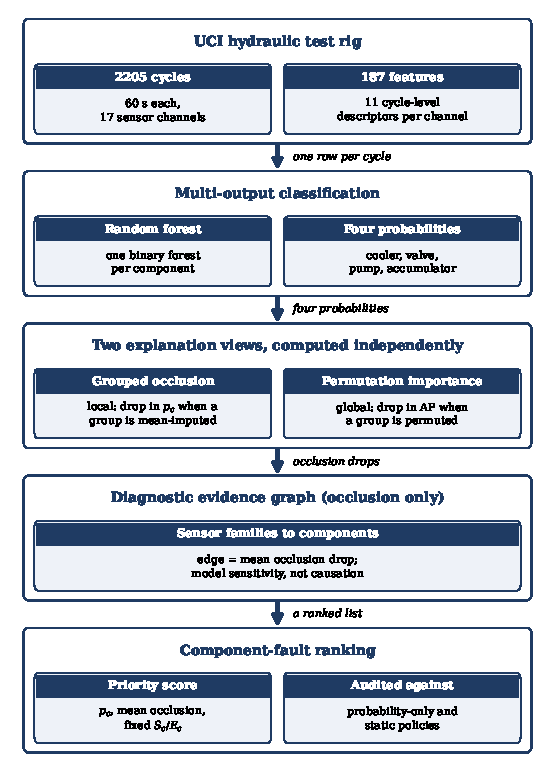
\includegraphics[width=\columnwidth]{paper3_conceptual_architecture.pdf}
    \caption{Implemented diagnostic workflow. The evidence graph and the priority
    score use grouped occlusion only.}
    \label{fig:architecture}
\end{figure}

\subsection{Multi-Output Classifier}
\label{sec:multioutput}

Let $x \in \R^d$ be the feature vector for one cycle and $y_c \in \{0,1\}$ the
fault state of component $c$. The classifier estimates
\begin{equation}
\begin{split}
p_c(x)&=P(y_c=1\mid x),\\
c &\in \{\text{cooler},\text{valve},\text{pump},\text{accumulator}\}.
\end{split}
\label{eq:probs}
\end{equation}
A random forest is fitted per component (260 trees, minimum leaf size 2, class
weights balanced per bootstrap sample, scikit-learn \texttt{MultiOutputClassifier})
on standardized features \cite{Breiman2001RF,Pedregosa2011Sklearn}. Its raw
probabilities are used throughout; no calibrator is fitted. Gradient-boosted
alternatives are competitive here \cite{Chen2016XGBoost,Ke2017LightGBM}, and
Sec.~\ref{sec:comparators} reports which conclusions change when one is used.

\subsection{Grouped Occlusion}
\label{sec:occlusion}

Grouped occlusion is a removal-based attribution \cite{Covert2021RemovalBased}. For
a feature group $s$ it replaces the group's standardized features with their
training-set mean, re-queries the model, and records the decrease:
\begin{equation}
a_{s,c}(x)=\max \left(p_c(x)-p_c(x_{\setminus s}),0\right).
\label{eq:occlusion}
\end{equation}
Groups are the 17 channels (11 features each) or the seven families of
Table~\ref{tab:channelmap}, in which all channels of a family are replaced at once.
A large value means that the model's output for that cycle is sensitive to the
group. Mean imputation creates inputs that may not occur on the rig, so $a_{s,c}$
measures model sensitivity under an artificial input. It is not, by itself,
evidence that the sensor physically reflects the fault.

\subsection{Permutation Importance}
\label{sec:permutation}

Permutation importance gives the global view of how much the fitted model relies on
a group across the held-out set \cite{Fisher2019ModelReliance}. For group $s$ and
component $c$,
\begin{equation}
I_{s,c}=\mathrm{AP}_c(f,X,Y)-\mathrm{AP}_c(f,X_{\pi(s)},Y),
\label{eq:permutation}
\end{equation}
where $X_{\pi(s)}$ is the held-out set with each feature of group $s$ independently
permuted, and negative drops are clipped to zero. The estimator is biased toward
correlated variables in tree ensembles \cite{Strobl2007Bias} and queries the model
off the data manifold \cite{Hooker2021Unrestricted}.

\subsection{Diagnostic Evidence Graph}
\label{sec:graph}

The graph has the seven sensor families and the four components as nodes. Its edge
weight is the mean family-level occlusion over the held-out cycles $X$,
\begin{equation}
w_{F,c}=\frac{1}{|X|}\sum_{x\in X} a_{F,c}(x),
\label{eq:edgeweight}
\end{equation}
where $F$ is a family occluded as one group. An edge is drawn when
$w_{F,c}\ge 0.01$, a mean drop of one percentage point in $p_c$, and its width is
proportional to $w_{F,c}$. The released graph (Fig.~\ref{fig:evidencegraph}) is an
aggregate over the pooled out-of-fold predictions of the blocked split, not a
single cycle. Permutation importance is not part of the edge weight. The graph
summarizes which sensor families the fitted model is sensitive to for each
component; it does not identify counterfactual effects, interventions or
structural equations.

Figure~\ref{fig:explanation} follows one sensor group and one component through
the two attribution views and shows what each view is used for.

\begin{figure}[!tbp]
    \centering
    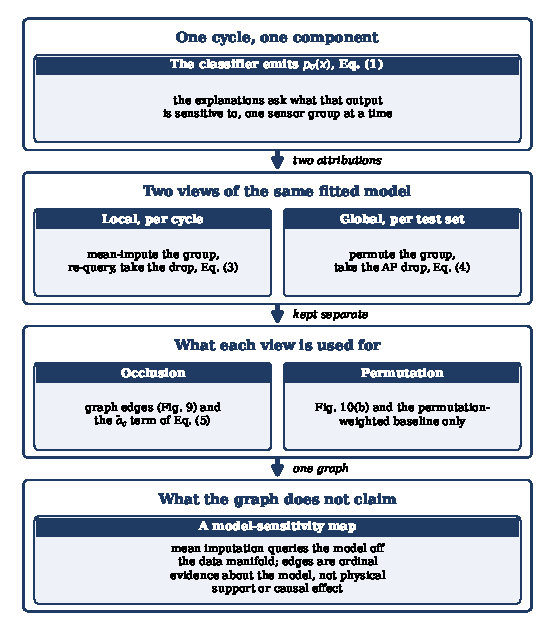
\includegraphics[width=\columnwidth]{paper3_explanation_evidence.pdf}
    \caption{The two attribution views. Occlusion supplies the graph edges and the $\bar a_c$ term of the priority score, while permutation importance is reported separately and used only by the permutation-weighted baseline.}
    \label{fig:explanation}
\end{figure}

\subsection{Maintenance-Priority Score}
\label{sec:priorityscore}

The component-priority score is
\begin{equation}
M_c(x)=p_c(x)\,(1+\bar{a}_c(x))\,\frac{S_c}{E_c},
\label{eq:priority}
\end{equation}
where $\bar{a}_c(x)$ is the mean of $a_{s,c}(x)$ over the 17 channel groups, and
$S_c$ and $E_c$ are severity and effort weights. The values used are in
Table~\ref{tab:constants}, and they are illustrative inputs chosen by the author to produce distinct
orderings, and they were not elicited from a maintenance organization or estimated
from cost records. Static severity-only, effort-only and severity-over-effort
policies are evaluated as baselines.

\begin{table}[t]
\centering
\caption{Severity ($S_c$) and effort ($E_c$) constants used by the priority score (Eq.~\ref{eq:priority}) and by the static policy baselines, read directly from \texttt{code/paper3\_diagnostics\_experiment.py}. The values are illustrative inputs chosen by the author to give distinct orderings, and they were not elicited from a maintenance organization or estimated from cost records.}
\label{tab:constants}
\footnotesize
\begin{tabular}{lrrr}
\hline
Component & $S_c$ & $E_c$ & $S_c/E_c$ \\
\hline
Cooler & 4.0 & 1.8 & 2.222 \\
Valve & 3.0 & 1.5 & 2.000 \\
Pump & 3.5 & 2.2 & 1.591 \\
Accumulator & 3.2 & 1.4 & 2.286 \\
\hline
\end{tabular}
\end{table}


Figure~\ref{fig:priorityrule} sets out the rule and the audit applied to it on the
leakage-safe blocked split (Sec.~\ref{sec:ceilingcheck}).

\begin{figure}[!tbp]
    \centering
    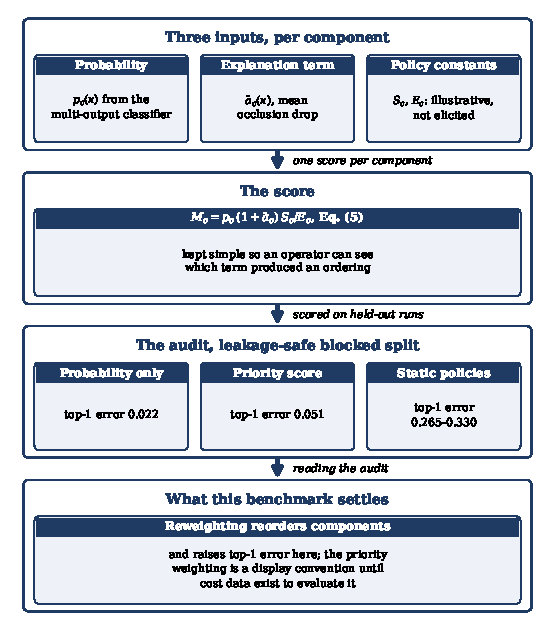
\includegraphics[width=\columnwidth]{paper3_priority_rule.pdf}
    \caption{The maintenance-priority rule and the audit applied to it. Error
    values are pooled out-of-fold top-1 component-fault errors on the blocked
    split (Table~\ref{tab:ceilingbound}).}
    \label{fig:priorityrule}
\end{figure}

\subsection{Separability Bound for Component-Fault Ranking}
\label{sec:ceiling}

Let $X$ be the fault-containing cycles of an evaluation set and, for $x\in X$, let
$P(x)=\{c:y_c=1\}$ and $N(x)=\{c:y_c=0\}$. A ranking policy assigns scores
$s_c(x)$ and ranks first the component with the largest score; ties are broken by
the fixed component order (cooler, valve, pump, accumulator), as \texttt{argmax}
does. The policy's top-1 error over the evaluation set is $E(s)=|X|^{-1}\sum_{x}\mathbf{1}[\text{first-ranked
component}\in N(x)]$, and we define
\begin{equation}
B(s)=\frac{1}{|X|}\sum_{x\in X}\sum_{c\in N(x)}\mathbf{1}\!\left[s_c(x)\ge\max_{q\in P(x)}s_q(x)\right].
\label{eq:unionbound}
\end{equation}

\begin{proposition}
\label{prop:bound}
(i) $E(s)\le B(s)$ for every score $s$. (ii) Let $p$ denote the probabilities of the classifier. If on every cycle $p_i(x)>p_j(x)$ implies $s_i(x)>s_j(x)$ (the score
preserves the classifier's strict per-cycle order; ties in $p$ may be broken
either way), then $E(s)\le B(s)\le B(p)$.
\end{proposition}
\begin{proof}
(i) If the first-ranked component $c^\ast$ of cycle $x$ is in $N(x)$, then
$s_{c^\ast}(x)\ge\max_{q\in P(x)}s_q(x)$, so the inner sum of \eqref{eq:unionbound}
is at least one on that cycle. (ii) If $p_c(x)<\max_{q\in P(x)}p_q(x)$, some true
positive $q$ has $p_q>p_c$, hence $s_q>s_c$ and the indicator for $s$ is zero.
Every indicator that is one for $s$ is therefore one for $p$.
\end{proof}

The cross-component AUC of component $c$ is
\begin{equation}
\mathrm{AUC}_c \;=\; \Pr\!\left[\max_{q\in P(x)} p_q(x) > p_c(x) \;\middle|\; c\in N(x)\right],
\label{eq:crossauc}
\end{equation}
estimated as the fraction of fault-containing cycles in which $c$ is a true
negative and the best true-positive probability exceeds $p_c$, with ties counted as
one-half. Grouping the terms of \eqref{eq:unionbound} by component gives the
reported bound,
\begin{equation}
B_p=\frac{1}{|X|}\sum_{x\in X}\;\sum_{c\in N(x)} \left(1-\mathrm{AUC}_c\right),
\label{eq:ceilingbound}
\end{equation}
which equals $B(p)$ except that a tie between a negative and the best positive
counts one-half instead of one. On every protocol reported here no such tie occurs
(Sec.~\ref{sec:ceilingcheck}), so $B_p=B(p)$ exactly.

Three consequences follow from the proposition, and the first is that $B_p$ is an upper limit on error; it need not be
attained, and $E(p)=B_p$ only when no cycle has two or more negatives at or above
its best positive. Second, $B_p$ covers a policy only on cycles where the policy
preserves the classifier's order. The local-occlusion score
$p_c(1+\bar a_c)$ and the priority score use component-specific factors, so they can
reorder components; for them only $B(s)$, computed from their own scores, is
guaranteed, and Sec.~\ref{sec:ceilingcheck} checks the order condition on every
cycle. Third, the bound is computed on the same evaluation set as the error, so its
value is diagnostic. It decomposes the ranking error of any order-preserving policy
into per-component cross-AUC terms, so a later study can read from the classifier
alone how much room a benchmark leaves for ranking policies to differ.

\section{Experimental Protocol}
\label{sec:protocol}

\subsection{Implementation}

The main script \nolinkurl{code/paper3_diagnostics_experiment.py} builds the
feature table, trains the classifier, computes attributions and writes the
random-split tables. \nolinkurl{code/leakage_robustness.py} evaluates the split
protocols, confusion matrices and noise stress. \nolinkurl{code/ceiling_analysis.py}
implements the bound, the chronological curve and the SHAP agreement check, and
\nolinkurl{code/run_clustered_bootstrap.py} replaces every interval with a
run-clustered one. \nolinkurl{code/degradation_walk.py} and
\nolinkurl{code/comparators.py} implement the degradation sweep and the classifier
comparators. The analyses added in revision (run-aligned purged blocks,
profile holdout, order-preservation checks, out-of-fold calibration, nested weight
selection, HistGradientBoosting ranking and attribution stability) are in
\nolinkurl{code/revision_analyses.py}, which first reproduces the published
blocked-split errors exactly as a control.

\subsection{Evaluation Protocols}
\label{sec:splits}

The 2205 cycles are indexed $i=0,\dots,2204$ in recording order, and five protocols
are reported. Each protocol supports a different claim \cite{Kaufman2012Leakage,Roberts2017CVStrategies}.
\begin{enumerate}
    \item The random stratified split holds out 30\% of cycles, stratified by whether
    any component is faulty (seed 17). Adjacent cycles of one run fall on both sides,
    so this split is an optimistic reference, and 656 of its 662 test cycles are
    fault-positive.
    \item The ten-block split assigns cycle $i$ to block $\min(\lfloor i/220\rfloor,9)$,
    which gives nine blocks of 220 cycles and one of 225. The scikit-learn
    \texttt{GroupKFold} splitter with five folds is deterministic and holds out two
    non-adjacent blocks per fold, $\{0,9\}$, $\{4,8\}$, $\{3,7\}$, $\{2,6\}$ and
    $\{1,5\}$, with no purge between training and test blocks. Because the block
    boundaries ignore condition-runs, 9 of the 194 runs straddle a boundary. As a
    result 18 held-out cycles are immediately adjacent to a training cycle, and 41\% of
    held-out cycles share their condition profile with a training run. This protocol
    therefore holds out contiguous time blocks, not whole runs or condition profiles.
    It produced the headline numbers of the original submission and is kept for
    continuity.
    \item The run-aligned purged split moves each of the nine interior block
    boundaries to the nearest start of a condition-run, so no run is split. For every
    held-out block, the runs immediately before and after it are also removed from
    training (20 to 30 cycles per fold), and no held-out cycle is adjacent to a
    training cycle. Held-out runs can still share a condition profile with a different
    training run (36\% of held-out cycles).
    \item Condition-profile holdout applies \texttt{GroupKFold} with five folds to the
    144 unique (cooler, valve, pump, accumulator) profiles. Every held-out profile is
    absent from training, although each component level occurs in training in other
    combinations. This protocol tests unseen fault combinations but does not control
    temporal adjacency, since 263 held-out cycles neighbor a training cycle of a
    different profile.
    \item The chronological split trains on the first 70\% of cycles and tests on the
    last 30\%. It is a stress test, because the final block contains no faulty cooler
    and few healthy accumulators \cite{MorenoTorres2012UnifyingView,Gama2014ConceptDrift}.
\end{enumerate}
None of these protocols evaluates future operation of a different rig, unseen
severity levels, or another asset. For the three cross-validated protocols,
macro-F1 is the mean over folds of the per-fold macro-F1, and ranking, calibration
and bound results use the pooled out-of-fold predictions of all 2205 cycles.

\subsection{Metrics}

Component classification is evaluated with accuracy, precision, recall, F1 and
average precision \cite{Davis2006PRvsROC,Saito2015PRPlot,Fawcett2006ROC}. When a
held-out set contains no positive case for a component, recall and F1 are
undefined. We report them as n/a and give positive and negative support. Macro-F1 is
reported over all four components, with an undefined F1 entered as 0 (the
scikit-learn \texttt{zero\_division=0} convention used in the original submission),
and also over the components whose F1 is defined. Probability reliability is evaluated
with the Brier score \cite{Brier1950Verification}, 10-bin expected calibration error
\cite{Naeini2015BayesianBinning,Guo2017Calibration}, and negative log loss.
Component-fault ranking is evaluated on cycles with at least one fault, using
label-ranking average precision (LRAP), top-1 accuracy (the first-ranked component
is truly faulty) and mean reciprocal rank (MRR)
\cite{Tsoumakas2007MultiLabel,Zhang2014MultiLabelReview}.

\subsection{Resampling Unit for Every Reported Interval}
\label{sec:resampling}

Every interval comes from a nonparametric bootstrap whose unit is the
\emph{condition-run}. Identical rows of \texttt{profile.txt} occur in contiguous
blocks, because the rig was set to a fault combination and left there for
consecutive load cycles. Grouping consecutive identical rows gives 194 runs, of which 36 have length 1, 154 have length 10, one has length 19, two have length 200 and one has length 210. Cycles inside a run share one configuration and a slowly drifting thermal
state, so a bootstrap that drew cycles independently would overstate the effective
sample size. On the blocked split the run-clustered intervals are 2.4 to 8.0 times
wider than cycle-level ones, and no point estimate changes. Where two policies are
compared on the same cycles, or a policy's error is compared with the bound, we
report a run-clustered \emph{paired} bootstrap of the difference (2{,}000
resamples). Whether two marginal intervals overlap is not used as a test.

\section{Results}
\label{sec:results}

\subsection{Component Classification and Leakage}

The random split produces near-perfect component metrics
(Table~\ref{tab:componentmetrics}, Fig.~\ref{fig:f1}), with macro-F1 0.999 and
every component above 0.99. Because adjacent cycles of the same run fall on both
sides of this split, it is read only as an optimistic reference.

\begin{figure}[!tbp]
    \centering
    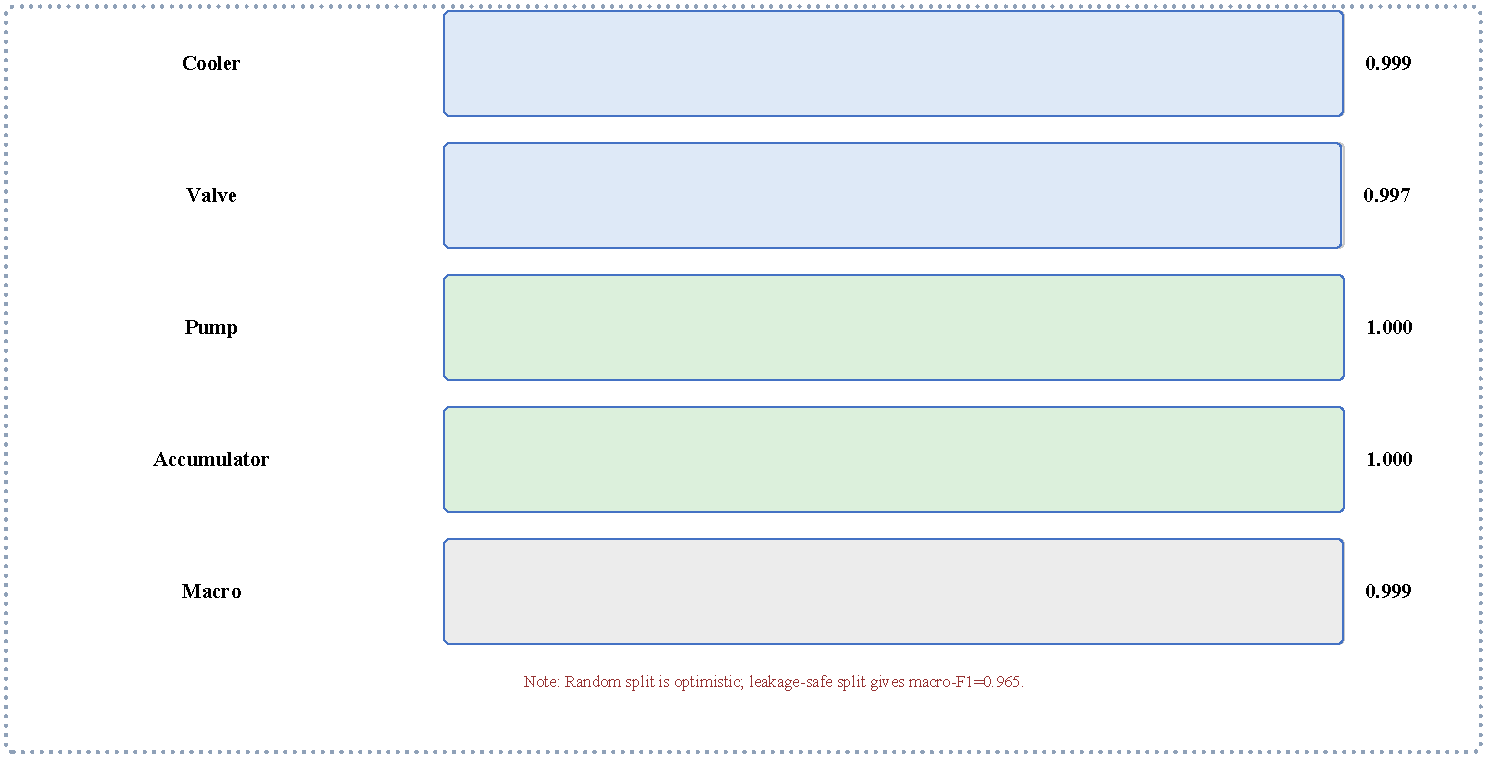
\includegraphics[width=\columnwidth]{paper3_component_f1.pdf}
    \caption{Random-split component F1 scores (optimistic reference).}
    \label{fig:f1}
\end{figure}

\begin{table*}[t]
\centering
\caption{Component fault classification metrics on the random stratified test split. This split is reported as an optimistic reference, and the leakage-controlled protocols are in Table~\ref{tab:splitcompare}.}
\label{tab:componentmetrics}
\footnotesize
\begin{tabular}{lrrrrr}
\toprule
Component & Accuracy & Precision & Recall & F1 & AP \\
\midrule
Cooler & 0.998 & 0.998 & 1.000 & 0.999 & 1.000 \\
Valve & 0.997 & 0.994 & 1.000 & 0.997 & 1.000 \\
Pump & 1.000 & 1.000 & 1.000 & 1.000 & 1.000 \\
Accumulator & 1.000 & 1.000 & 1.000 & 1.000 & 1.000 \\
\midrule
\textbf{Macro} & \textbf{0.999} & \textbf{0.998} & \textbf{1.000} & \textbf{0.999} & \textbf{1.000} \\
\bottomrule
\end{tabular}
\end{table*}


Table~\ref{tab:splitcompare} reports the leakage-controlled protocols with
per-component support, and Fig.~\ref{fig:splitsensitivity} shows them side by side.
Macro-F1 is 0.965 on the ten-block split, 0.962 after run alignment and purging,
and 0.963 under condition-profile holdout. The purge costs mainly the valve (F1
0.991 to 0.964); the accumulator is the hardest component under every
leakage-controlled protocol (F1 0.888 to 0.900). These results support performance
on held-out runs and on fault combinations that were absent from training, on this
rig. They do not establish performance under future operation, at unseen severity
levels, or on another rig.

\begin{table*}[t]
\centering
\caption{Component-fault classification under four evaluation protocols. Per-component F1 is computed on pooled held-out predictions for seed 2026, and macro-F1 is the mean over folds of the per-fold macro-F1, averaged over the stated seeds. Positive and negative test support is given in parentheses. F1 is reported as n/a when the held-out set contains no positive case, because recall is then undefined, and ``Macro-F1, defined'' averages only the components whose F1 is defined in each fold. The last column gives the share of held-out cycles whose condition profile also occurs in training and the number of held-out cycles immediately adjacent in time to a training cycle.}
\label{tab:splitcompare}
\footnotesize
\setlength{\tabcolsep}{3pt}
\resizebox{\linewidth}{!}{%
\begin{tabular}{lrrrrrrrr}
\toprule
Protocol & Seeds & Macro-F1 & Macro-F1, & Cooler & Valve & Pump & Accum. & Profile in train / \\
 & & (all 4) & defined & F1 (+/$-$) & F1 (+/$-$) & F1 (+/$-$) & F1 (+/$-$) & adjacent cycles \\
\midrule
Blocked (original, 10 equal blocks) & 2 & 0.965 & 0.965 & 0.995 (1464/741) & 0.991 (1080/1125) & 0.993 (984/1221) & 0.888 (1606/599) & 0.41 / 18 \\
Blocked, run-aligned + purged & 3 & 0.962 & 0.962 & 0.995 (1464/741) & 0.964 (1080/1125) & 0.993 (984/1221) & 0.896 (1606/599) & 0.36 / 0 \\
Condition-profile holdout & 3 & 0.963 & 0.963 & 0.994 (1464/741) & 0.970 (1080/1125) & 0.998 (984/1221) & 0.900 (1606/599) & 0.00 / 263 \\
Chronological 70/30 & 1 & 0.667 & 0.890 & n/a (0/662) & 0.786 (360/302) & 0.995 (328/334) & 0.888 (529/133) & 0.23 / 1 \\
\bottomrule
\end{tabular}}
\end{table*}


\begin{figure*}[!t]
    \centering
    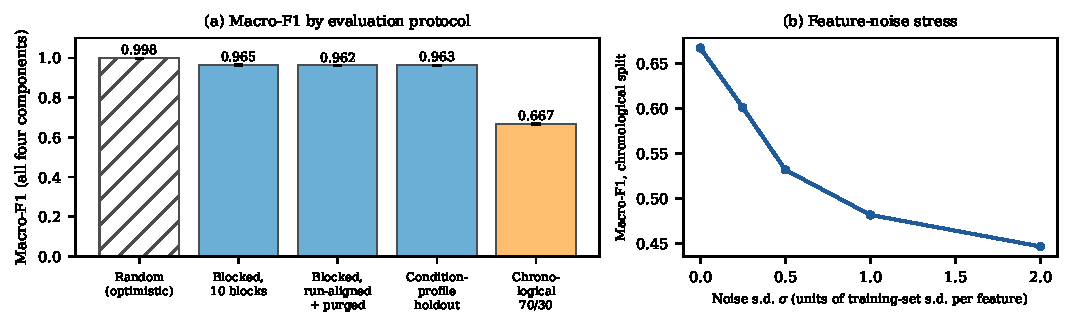
\includegraphics[width=0.85\textwidth]{paper3_split_sensitivity.pdf}
    \caption{Split sensitivity. (a) Macro-F1 over all four components under five protocols, with error bars giving the standard deviation over seeds. The hatched random-split bar is an optimistic reference. (b) Chronological-split macro-F1 as zero-mean Gaussian noise is added to the standardized test features, where $\sigma$ is in units of each feature's training-set standard deviation.}
    \label{fig:splitsensitivity}
\end{figure*}

The chronological split is a separate stress test (Tables~\ref{tab:leakage_robustness}
and~\ref{tab:confusion}). Its test block has no faulty cooler (0 of 662 cycles),
so cooler F1 is undefined. Entered as 0 it gives the macro-F1 of 0.667 reported in
the original submission; over the three components with defined F1 the value is
0.890. The two figures are not comparable with the cross-validated protocols, where
every component has both classes. The accumulator shows the opposite failure, with no true negatives among 133 healthy accumulator cycles, because a fault is predicted
for every cycle of the final block. Table~\ref{tab:leakage_robustness} also gives a
noise stress test on this split, in which noise is added to features after
standardization by the training mean and standard deviation, so $\sigma=1$ equals
one training standard deviation of each feature.

\begin{table*}[t]
\centering
\caption{Split robustness and noise stress for the diagnostics model (macro-F1 over all four components). The random split is an optimistic reference, the ten-block split is the leakage-controlled protocol of the original submission, and the strict chronological split exposes strong distribution shift in the final cycles. Sensor-noise rows are measured on the chronological split. The random-split row is recomputed with an independently retrained model (seed 2026), so it differs by ordinary seed variance from the seed-17 model behind Table~\ref{tab:componentmetrics} (0.998 here and 0.999 there).}
\label{tab:leakage_robustness}
\begin{tabular}{lr}
\toprule
Evaluation & Macro-F1 \\
\midrule
\multicolumn{2}{l}{\emph{Split protocol}} \\
Random stratified split (optimistic reference) & 0.998 \\
Blocked group 5-fold split (leakage-safe headline) & \textbf{0.965} \\
Temporal chronological split (strict stress test) & 0.667 \\
\midrule
\multicolumn{2}{l}{\emph{Sensor-noise stress, chronological split}} \\
Temporal split, sensor noise $\sigma=0.00$ & 0.667 \\
Temporal split, sensor noise $\sigma=0.25$ & 0.601 \\
Temporal split, sensor noise $\sigma=0.50$ & 0.532 \\
Temporal split, sensor noise $\sigma=1.00$ & 0.482 \\
Temporal split, sensor noise $\sigma=2.00$ & 0.447 \\
\bottomrule
\end{tabular}
\end{table*}

\begin{table*}[t]
\centering
\caption{Per-component confusion matrices under the strict chronological split (TN/FP/FN/TP and F1). Two entries are degenerate. The cooler has no positive cases in the final block, so its recall and F1 are undefined (n/a), and the 0.667 macro-F1 of Table~\ref{tab:leakage_robustness} enters it as 0 by the scikit-learn \texttt{zero\_division=0} convention. The accumulator has no true negatives, because a fault is predicted for every cycle.}
\label{tab:confusion}
\begin{tabular}{lrrrrr}
\toprule
Component & TN & FP & FN & TP & F1 \\
\midrule
Cooler & 662 & 0 & 0 & 0 & n/a \\
Valve & 302 & 0 & 127 & 233 & 0.786 \\
Pump & 334 & 0 & 3 & 325 & 0.995 \\
Accumulator & 0 & 133 & 0 & 529 & 0.888 \\
\bottomrule
\end{tabular}
\end{table*}


\subsection{Probability Calibration}

No calibrator is fitted, so the priority score consumes raw forest probabilities.
On the random split they look well calibrated (Table~\ref{tab:calibration}; macro
Brier 0.0031, macro ECE 0.0202), but that split is optimistic and is a best case.
Table~\ref{tab:calibrationoof} and Fig.~\ref{fig:reliability} give calibration on
pooled out-of-fold predictions of the leakage-controlled protocols. On the blocked
split the cooler (ECE 0.005) and pump (0.021) remain well calibrated, the valve is
not (0.097), and the accumulator is worst (Brier 0.136, ECE 0.113), with a mean
predicted probability of 0.786 against an observed fault rate of 0.728. Macro Brier
rises to 0.042 and macro ECE to 0.059. The probabilities that enter the priority
score are therefore reliable for two components and unreliable for the two that
drive most ranking errors. Recalibration by Platt scaling or isotonic regression
\cite{Platt1999Probabilistic,NiculescuMizil2005Predicting}, fitted inside each
training fold, would be required before the probabilities are used as risks.

\begin{table}[t]
\centering
\caption{Calibration of the raw random-forest probabilities on the random stratified test split (seed 17), with no calibrator fitted. This split is optimistic, so these values are a best case, and leakage-safe values are in Table~\ref{tab:calibrationoof}.}
\label{tab:calibration}
\footnotesize
\begin{tabular}{lrrrrr}
\toprule
Component & Pos. rate & Mean $p$ & Brier $\downarrow$ & ECE $\downarrow$ & NLL $\downarrow$ \\
\midrule
Cooler & 0.690 & 0.691 & 0.0012 & 0.0021 & 0.0035 \\
Valve & 0.503 & 0.506 & 0.0063 & 0.0401 & 0.0479 \\
Pump & 0.459 & 0.459 & 0.0005 & 0.0060 & 0.0063 \\
Accumulator & 0.728 & 0.725 & 0.0043 & 0.0329 & 0.0355 \\
\midrule
\textbf{Macro} & 0.595 & 0.595 & \textbf{0.0031} & \textbf{0.0202} & \textbf{0.0233} \\
\bottomrule
\end{tabular}
\end{table}

\begin{table}[t]
\centering
\caption{Calibration of the raw random-forest probabilities (no calibrator is fitted) on pooled out-of-fold predictions for the three leakage-controlled protocols, seed 2026. The intervals in brackets are run-clustered 95\% intervals from 1{,}000 resamples.}
\label{tab:calibrationoof}
\footnotesize
\setlength{\tabcolsep}{2pt}
\resizebox{\linewidth}{!}{%
\begin{tabular}{llrll}
\toprule
Protocol & Comp. & Pos. & Brier [95\% CI] & ECE [95\% CI] \\
\midrule
Blocked (orig.) & Cooler & 0.66 & 0.004 [0.000, 0.008] & 0.005 [0.002, 0.013] \\
 & Valve & 0.49 & 0.024 [0.017, 0.033] & 0.097 [0.077, 0.118] \\
 & Pump & 0.45 & 0.005 [0.002, 0.010] & 0.021 [0.015, 0.028] \\
 & Accumulator & 0.73 & 0.136 [0.099, 0.184] & 0.113 [0.076, 0.171] \\
\midrule
Blocked, purged & Cooler & 0.66 & 0.005 [0.000, 0.009] & 0.005 [0.002, 0.015] \\
 & Valve & 0.49 & 0.043 [0.031, 0.056] & 0.115 [0.095, 0.147] \\
 & Pump & 0.45 & 0.007 [0.004, 0.011] & 0.038 [0.029, 0.048] \\
 & Accumulator & 0.73 & 0.135 [0.101, 0.179] & 0.089 [0.059, 0.151] \\
\midrule
Profile holdout & Cooler & 0.66 & 0.006 [0.000, 0.011] & 0.004 [0.001, 0.022] \\
 & Valve & 0.49 & 0.042 [0.027, 0.061] & 0.108 [0.078, 0.154] \\
 & Pump & 0.45 & 0.002 [0.001, 0.004] & 0.019 [0.011, 0.029] \\
 & Accumulator & 0.73 & 0.111 [0.033, 0.232] & 0.080 [0.040, 0.245] \\
\bottomrule
\end{tabular}}
\end{table}


\begin{figure*}[!t]
    \centering
    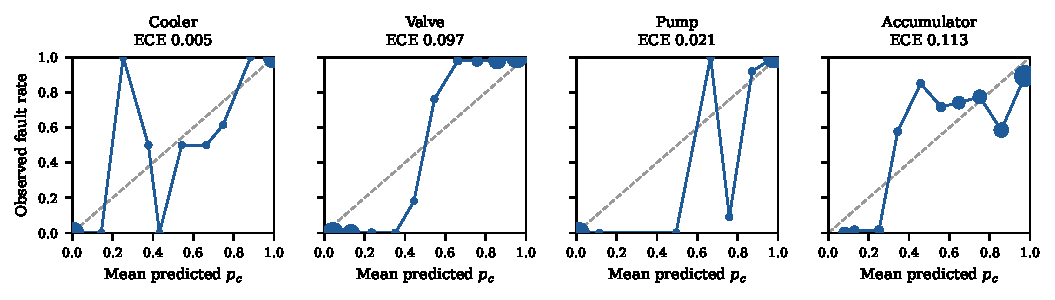
\includegraphics[width=0.85\textwidth]{rev_reliability_blocked.pdf}
    \caption{Reliability diagrams on pooled out-of-fold predictions of the blocked split (seed 2026), with 10 equal-width bins and marker area proportional to bin count.}
    \label{fig:reliability}
\end{figure*}

\subsection{Component-Fault Ranking on the Random Split}

Table~\ref{tab:ranking} and Fig.~\ref{fig:ranking} give the random-split ranking
comparison. Probability-only, permutation-weighted, local-occlusion and full
priority scores all reach LRAP, top-1 and MRR of 1.000; the static severity-only,
low-effort-only and severity/effort policies reach top-1 between 0.697 and 0.735.
On this split every policy that reads the probabilities saturates, so the split can
separate consulting the classifier from ignoring it but cannot separate the ways of
combining its outputs.

\begin{figure}[!tbp]
    \centering
    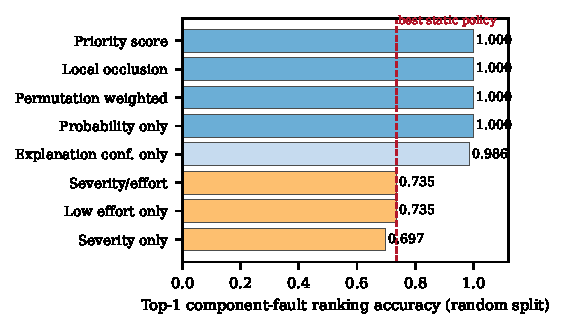
\includegraphics[width=\columnwidth]{paper3_root_cause_ranking.pdf}
    \caption{Top-1 component-fault ranking accuracy on the random split.}
    \label{fig:ranking}
\end{figure}

\begin{table*}[t]
\centering
\caption{Component-fault ranking on fault-containing test cycles of the random split (optimistic reference). Top-1 is the share of cycles whose first-ranked component is truly faulty. Static policies are included to test whether the priority rule adds information beyond the severity and effort constants. The leakage-safe comparison is in Tables~\ref{tab:ceilingbound} and~\ref{tab:boundcheck}.}
\label{tab:ranking}
\footnotesize
\begin{tabularx}{\textwidth}{Xrrr}
\toprule
Method & LRAP & Top-1 & MRR \\
\midrule
\multicolumn{4}{l}{\emph{Static policy baselines (do not use classifier probabilities)}} \\
Severity-only policy & 0.781 & 0.697 & 0.821 \\
Low-effort-only policy & 0.805 & 0.735 & 0.845 \\
Severity/effort heuristic & 0.837 & 0.735 & 0.859 \\
\midrule
\multicolumn{4}{l}{\emph{Explanation-only}} \\
Explanation confidence only & 0.984 & 0.986 & 0.993 \\
\midrule
\multicolumn{4}{l}{\emph{Probability-informed policies (all saturate on this split)}} \\
Probability only & 1.000 & 1.000 & 1.000 \\
Permutation weighted & 1.000 & 1.000 & 1.000 \\
Local occlusion & 1.000 & 1.000 & 1.000 \\
Priority score (prob.\ $+$ evidence $+$ severity/effort) & 1.000 & 1.000 & 1.000 \\
\bottomrule
\end{tabularx}
\end{table*}


\subsection{Leakage-Safe Ranking and the Bound}
\label{sec:ceilingcheck}

Table~\ref{tab:ceilingbound} gives the observed top-1 error of every policy against
$B_p$ on the random, blocked and chronological splits, and
Fig.~\ref{fig:ceilingbound} draws the same values. Table~\ref{tab:boundcheck} adds
the two new protocols, the bound $B_s$ computed from each policy's own score, and
the order-preservation check of Proposition~\ref{prop:bound}.
The paired differences are in Table~\ref{tab:paireddiff}.

On the blocked split, probability-only ranking has error 0.022 against $B_p=0.023$;
the paired difference $E-B_p$ is $-0.0005$ [$-0.001$, 0.000], so the bound is
attained to within one cycle in a thousand. The probabilities tie at the top on 204
fault-containing cycles, but every tie is between two true positives, so tie
handling changes neither the error nor the bound. Local occlusion (0.028) and the
full priority score (0.051) lie above $B_p$, by $+0.005$ [0.001, 0.012] and
$+0.028$ [0.012, 0.051]. Neither is covered by Proposition~\ref{prop:bound}(ii), because local occlusion violates the classifier's strict order on 16.9\% of cycles and the
priority score on 54.9\%. The claim in the original submission that local occlusion
satisfies the bound's condition was incorrect and is withdrawn. Both policies stay
below their own bound $B_s$, as part (i) requires.

The comparison behind the paper's negative result is the full priority score
against probability-only ranking, scored on the same cycles. On the ten-block split
the priority score's error is higher by 0.029 [0.012, 0.052]. The difference has the
same sign for all ten seeds of Table~\ref{tab:reconcile}, ranging from 0.025 to
0.034. On the run-aligned purged split it is 0.021 [0.008, 0.040]. On the 566
single-fault cycles, where top-1 accuracy is identification of the one faulted
component, the errors are 0.039 and 0.071 (ten blocks) and 0.049 and 0.092 (purged)
(\texttt{results/revision/single\_fault\_subset.csv}). Under condition-profile holdout the difference vanishes, at 0.001 [$-$0.001, 0.003] with probability-only error 0.006.
On the chronological split every probability-based policy has error 0.175 and
lands on $B_p$. The negative result is therefore specific to the temporally blocked
protocols, where the classifier makes enough errors for the reweighting to matter.
The three static policies remain far above the bound on every protocol (0.265 to
0.330 on the blocked split).

\begin{figure}[!tbp]
    \centering
    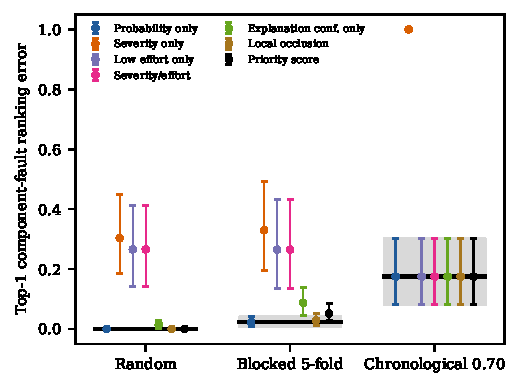
\includegraphics[width=\columnwidth]{ceiling_bound_vs_observed.pdf}
    \caption{Observed top-1 component-fault error for every policy against the probability-derived bound $B_p$ (black bar, with the run-clustered 95\% interval shaded) on three splits. $B_p$ covers only order-preserving policies (Proposition~\ref{prop:bound}). Values are from \texttt{results/ceiling\_bound\_check\_runclustered.csv}.}
    \label{fig:ceilingbound}
\end{figure}

\begin{table}[t]
\centering
\caption{Probability-derived union bound $B_p$ on top-1 component-fault ranking error (Sec.~\ref{sec:ceiling}) against each policy's observed top-1 error, with 2{,}000-resample bootstrap 95\% intervals in brackets. The bootstrap resamples whole condition-runs, which are the 194 contiguous blocks of cycles sharing one \texttt{profile.txt} row (Sec.~\ref{sec:resampling}). The last column marks whether the point estimate of the error is at or below that of $B_p$, and it is descriptive only. Whether a policy differs from the bound is tested with the paired intervals of Table~\ref{tab:paireddiff}, and $B_p$ is guaranteed to cover only order-preserving policies (Proposition~\ref{prop:bound}). The blocked rows pool the out-of-fold predictions of all five folds (2205 cycles, seed 2026). ``Priority score'' is Eq.~\eqref{eq:priority}. Code is in \texttt{code/run\_clustered\_bootstrap.py} and data in \texttt{results/ceiling\_bound\_check\_runclustered.csv}.}
\label{tab:ceilingbound}
\tiny
\setlength{\tabcolsep}{2pt}
\begin{tabular}{p{1.35cm}p{1.85cm}p{1.75cm}p{1.75cm}p{0.5cm}}
\hline
 Split & Policy & Obs.\ error & Bound $B_p$ & $E\le B_p$ \\
 & & [95\% CI] & [95\% CI] & (point) \\
\hline
Random & Probability only & 0.000 [0.000, 0.000] & 0.000 [0.000, 0.000] & Y \\
Random & Severity only & 0.303 [0.186, 0.448] & 0.000 [0.000, 0.000] & N \\
Random & Low effort only & 0.265 [0.142, 0.412] & 0.000 [0.000, 0.000] & N \\
Random & Severity/effort & 0.265 [0.142, 0.412] & 0.000 [0.000, 0.000] & N \\
Random & Explanation conf.\ only & 0.014 [0.001, 0.028] & 0.000 [0.000, 0.000] & N \\
Random & Local occlusion & 0.000 [0.000, 0.000] & 0.000 [0.000, 0.000] & Y \\
Random & Priority score & 0.000 [0.000, 0.000] & 0.000 [0.000, 0.000] & Y \\
\hline
Blocked 5-fold & Probability only & 0.022 [0.009, 0.040] & 0.023 [0.009, 0.040] & Y \\
Blocked 5-fold & Severity only & 0.330 [0.194, 0.492] & 0.023 [0.009, 0.040] & N \\
Blocked 5-fold & Low effort only & 0.265 [0.134, 0.433] & 0.023 [0.009, 0.040] & N \\
Blocked 5-fold & Severity/effort & 0.265 [0.134, 0.433] & 0.023 [0.009, 0.040] & N \\
Blocked 5-fold & Explanation conf.\ only & 0.087 [0.044, 0.138] & 0.023 [0.009, 0.040] & N \\
Blocked 5-fold & Local occlusion & 0.028 [0.012, 0.051] & 0.023 [0.009, 0.040] & N \\
Blocked 5-fold & Priority score & 0.051 [0.027, 0.084] & 0.023 [0.009, 0.040] & N \\
\hline
Chronological & Probability only & 0.175 [0.080, 0.301] & 0.175 [0.080, 0.301] & Y \\
Chronological & Severity only & 1.000 [1.000, 1.000] & 0.175 [0.080, 0.301] & N \\
Chronological & Low effort only & 0.175 [0.080, 0.301] & 0.175 [0.080, 0.301] & Y \\
Chronological & Severity/effort & 0.175 [0.080, 0.301] & 0.175 [0.080, 0.301] & Y \\
Chronological & Explanation conf.\ only & 0.175 [0.080, 0.301] & 0.175 [0.080, 0.301] & Y \\
Chronological & Local occlusion & 0.175 [0.080, 0.301] & 0.175 [0.080, 0.301] & Y \\
Chronological & Priority score & 0.175 [0.080, 0.301] & 0.175 [0.080, 0.301] & Y \\
\hline
\end{tabular}
\end{table}

\begin{table*}[t]
\centering
\caption{Top-1 component-fault ranking error on fault-containing held-out cycles, the probability-derived union bound $B_p$ of \eqref{eq:ceilingbound}, and the order-preservation check of Proposition~\ref{prop:bound}. ``Violation'' is the share of cycles with at least one pair $i,j$ such that $p_i>p_j$ but $s_i\le s_j$, and $B_p$ is guaranteed to cover a policy only when this share is zero. ``Top-1 = prob.'' is the share of cycles on which the policy's first-ranked component is the same as that of probability-only ranking. $B_s$ is the bound recomputed from the policy's own score with ties counted as misranks, and it holds for every policy by construction. All values are for seed 2026, with run-clustered 95\% intervals from 2{,}000 resamples.}
\label{tab:boundcheck}
\footnotesize
\setlength{\tabcolsep}{3pt}
\resizebox{\linewidth}{!}{%
\begin{tabular}{llrlrrrr}
\toprule
Protocol & Policy & Error & [95\% CI] & $B_p$ & $B_s$ & Violation & Top-1 = prob. \\
\midrule
Blocked (original) & Probability only & 0.022 & [0.009, 0.040] & 0.023 & 0.023 & 0.000 & 1.000 \\
 & Local occlusion & 0.028 & [0.012, 0.051] & 0.023 & 0.029 & 0.169 & 0.799 \\
 & Priority score & 0.051 & [0.027, 0.084] & 0.023 & 0.052 & 0.549 & 0.567 \\
 & Severity/effort & 0.265 & [0.134, 0.433] & 0.023 & 0.326 & 0.953 & 0.166 \\
\midrule
Blocked, run-aligned + purged & Probability only & 0.031 & [0.014, 0.053] & 0.032 & 0.032 & 0.000 & 1.000 \\
 & Local occlusion & 0.034 & [0.016, 0.058] & 0.032 & 0.035 & 0.203 & 0.791 \\
 & Priority score & 0.051 & [0.028, 0.084] & 0.032 & 0.052 & 0.498 & 0.652 \\
 & Severity/effort & 0.265 & [0.134, 0.433] & 0.032 & 0.326 & 0.984 & 0.178 \\
\midrule
Condition-profile holdout & Probability only & 0.006 & [0.000, 0.014] & 0.007 & 0.007 & 0.000 & 1.000 \\
 & Local occlusion & 0.006 & [0.000, 0.014] & 0.007 & 0.007 & 0.187 & 0.712 \\
 & Priority score & 0.007 & [0.001, 0.015] & 0.007 & 0.008 & 0.505 & 0.557 \\
 & Severity/effort & 0.265 & [0.134, 0.433] & 0.007 & 0.326 & 0.956 & 0.157 \\
\midrule
Chronological 70/30 & Probability only & 0.175 & [0.080, 0.301] & 0.175 & 0.175 & 0.000 & 1.000 \\
 & Local occlusion & 0.175 & [0.080, 0.301] & 0.175 & 0.175 & 0.000 & 1.000 \\
 & Priority score & 0.175 & [0.080, 0.301] & 0.175 & 0.175 & 0.111 & 1.000 \\
 & Severity/effort & 0.175 & [0.080, 0.301] & 0.175 & 0.384 & 0.749 & 1.000 \\
\bottomrule
\end{tabular}}
\end{table*}

\begin{table}[t]
\centering
\caption{Run-clustered paired bootstrap differences for seed 2026 (2{,}000 resamples, 95\% intervals). $\Delta_{\mathrm{prio}}$ is the priority-score error minus the probability-only error, and $E-B_p$ is a policy's error minus the probability-derived bound, both computed on the same resample.}
\label{tab:paireddiff}
\footnotesize
\setlength{\tabcolsep}{2pt}
\begin{tabular}{lll}
\toprule
Protocol & Quantity & Estimate [95\% CI] \\
\midrule
Blocked (orig.) & $\Delta_{\mathrm{prio}}$ & +0.029 [0.012, 0.052] \\
 & $E-B_p$, prob.\ only & -0.000 [-0.001, 0.000] \\
 & $E-B_p$, local occl. & +0.005 [0.001, 0.012] \\
 & $E-B_p$, priority & +0.028 [0.012, 0.051] \\
\midrule
Blocked, purged & $\Delta_{\mathrm{prio}}$ & +0.021 [0.008, 0.040] \\
 & $E-B_p$, prob.\ only & -0.001 [-0.003, 0.000] \\
 & $E-B_p$, local occl. & +0.002 [-0.001, 0.007] \\
 & $E-B_p$, priority & +0.020 [0.007, 0.039] \\
\midrule
Profile holdout & $\Delta_{\mathrm{prio}}$ & +0.001 [-0.001, 0.003] \\
 & $E-B_p$, prob.\ only & -0.000 [-0.001, 0.000] \\
 & $E-B_p$, local occl. & -0.000 [-0.001, 0.000] \\
 & $E-B_p$, priority & +0.000 [-0.001, 0.003] \\
\midrule
Chronological & $\Delta_{\mathrm{prio}}$ & +0.000 [0.000, 0.000] \\
 & $E-B_p$, prob.\ only & +0.000 [-0.000, 0.000] \\
 & $E-B_p$, local occl. & +0.000 [-0.000, 0.000] \\
 & $E-B_p$, priority & +0.000 [-0.000, 0.000] \\
\bottomrule
\end{tabular}
\end{table}

\begin{table}[t]
\centering
\caption{Cross-component AUC per component and split, defined as the probability that the best true-positive component's score exceeds this component's score on fault-containing cycles where it is a true negative.}
\label{tab:crossauc}
\footnotesize
\begin{tabular}{llrr}
\hline
Split & Component & Cross-AUC & $n$ cycles \\
\hline
Random & Cooler & 1.000 & 199 \\
Random & Valve & 1.000 & 323 \\
Random & Pump & 1.000 & 352 \\
Random & Accumulator & 1.000 & 174 \\
\hline
Blocked 5-fold & Cooler & 0.996 & 720 \\
Blocked 5-fold & Valve & 0.999 & 1104 \\
Blocked 5-fold & Pump & 1.000 & 1200 \\
Blocked 5-fold & Accumulator & 0.920 & 578 \\
\hline
Chronological & Cooler & 1.000 & 641 \\
Chronological & Valve & 1.000 & 281 \\
Chronological & Pump & 1.000 & 313 \\
Chronological & Accumulator & 0.000 & 112 \\
\hline
\end{tabular}
\end{table}


Table~\ref{tab:crossauc} gives the per-component cross-AUC, and on the random split every component reaches 1.000, so $B_p=0$. On the blocked split the accumulator
falls to 0.920, which accounts for most of $B_p=0.023$. On the chronological split
accumulator cross-AUC is 0.000. Whenever the accumulator is healthy and another component is faulted, its probability is never below the best true positive's, and this single component sets $B_p=0.175$. Severity-only ranking has error
1.000 there, because it always ranks the cooler first and the cooler has no faults in
the test block.

\subsection{Chronological Generalization Curve}
\label{sec:chronocurve}

The single 70\% cut reports one point on a curve. We retrain at nine cut points,
from 50\% to 90\% in steps of five percentage points, and recompute cross-AUC and
every policy's top-1 accuracy (Table~\ref{tab:chronocurve},
Fig.~\ref{fig:chronocurve}). Mean cross-AUC is 0.683 at the 50\% cut, 0.750 at
70\%, and 1.000 from 80\% onward, so separability depends on which fault states fall
in the test tail. Between the 50\% and 65\% cuts the training fold contains no
healthy cooler, the cooler model degenerates to a constant probability of 1.0, and
every score that includes that probability ranks the cooler first. Probability-only,
local-occlusion and priority scores fall to top-1 accuracy between 0.041 and 0.335,
while the severity/effort and low-effort policies, which rank the accumulator first,
reach 0.79 to 0.90 because the accumulator is the majority faulted component in
those tails. This is a base-rate match between a constant ranking and a locally
dominant fault class, coincident with a training-fold pathology. From the 70\% cut
onward probability-only and the priority score move together.

\begin{figure*}[!t]
    \centering
    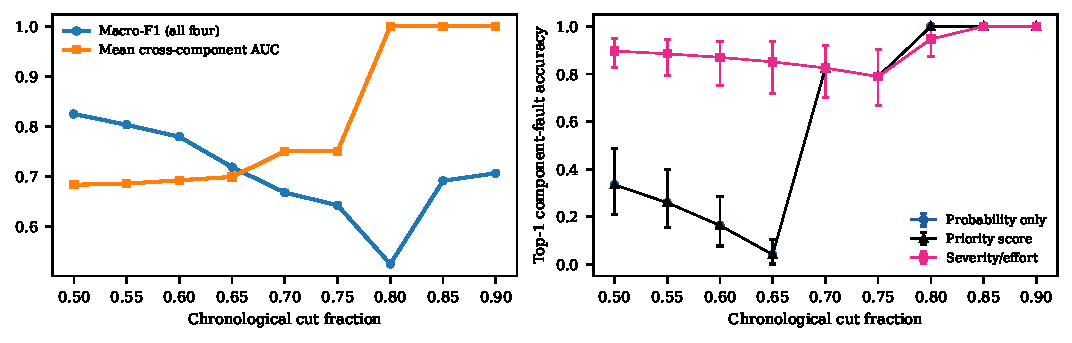
\includegraphics[width=0.85\textwidth]{ceiling_chronological_curve.pdf}
    \caption{Chronological generalization curve. The left panel gives macro-F1 and mean cross-component AUC at nine cut points, and the right panel gives the top-1 component-fault accuracy of three policies with 95\% run-clustered intervals (500 resamples per point). Values are from \texttt{results/chronological\_curve\_runclustered.csv}.}
    \label{fig:chronocurve}
\end{figure*}

\begin{table}[t]
\centering
\caption{Chronological generalization curve, giving macro-F1, mean cross-component AUC and the top-1 component-fault ranking accuracy of two policies as the cut point moves later in the cycle sequence. All rows use seed 2026, and the 0.70 row matches Table~\ref{tab:leakage_robustness}. At cut points 0.50 to 0.65 the cooler training fold contains no healthy cooler (Sec.~\ref{sec:chronocurve}), so the cooler classifier degenerates to a constant score. This lowers every score that includes it and is a training-fold pathology of the early cuts, not evidence about ranking quality.}
\label{tab:chronocurve}
\footnotesize
\setlength{\tabcolsep}{4pt}
\begin{tabular}{rrrrr}
\hline
Cut & Macro-F1 & Mean & Top-1 & Top-1 \\
 & & cross-AUC & prob.\ only & priority \\
\hline
0.50 & 0.825 & 0.683 & 0.335 & 0.335 \\
0.55 & 0.803 & 0.685 & 0.259 & 0.259 \\
0.60 & 0.779 & 0.692 & 0.164 & 0.164 \\
0.65 & 0.718 & 0.699 & 0.041 & 0.041 \\
0.70 & 0.667 & 0.750 & 0.825 & 0.825 \\
0.75 & 0.642 & 0.750 & 0.789 & 0.789 \\
0.80 & 0.524 & 1.000 & 1.000 & 1.000 \\
0.85 & 0.691 & 1.000 & 1.000 & 1.000 \\
0.90 & 0.706 & 1.000 & 1.000 & 1.000 \\
\hline
\end{tabular}
\end{table}


\subsection{Priority-Weight Sensitivity}
\label{sec:sensitivity}

The weight analysis of the original submission used the random split, where every
probability-based variant saturates at top-1 1.000, so it could not show whether a
weighting helps. Table~\ref{tab:sensitivity} repeats it on the pooled out-of-fold
predictions of the blocked split for the score $p_c(1+\gamma\bar a_c)S_c^a/E_c^b$.
Every scenario of the original analysis has higher error than probability-only
ranking, by 0.006 for the evidence term alone and by 0.017 to 0.030 for every
variant that includes severity and effort.

A wider 48-point grid ($\gamma\in\{0,0.5,1,2\}$, $a\in\{0,0.5,1,1.5\}$,
$b\in\{0,0.5,1\}$; \texttt{results/revision/weight\_grid\_blocked.csv}) shows that
this is not the whole picture. Read with hindsight on the evaluation split, 11
settings have lower error than probability-only ranking, all with $b=0$; the best,
$a=1.5$ and $\gamma=0$, reaches 0.008. Those settings raise the cooler and pump relative to the accumulator, whose healthy
cycles are the ones most often outscored by a faulted component (cross-AUC 0.920,
Table~\ref{tab:crossauc}). The advantage disappears once the weights are selected without the evaluation data. When $(\gamma,a,b)$ is chosen
by four-fold group cross-validation on the training blocks of each outer fold and
scored on the held-out blocks, the selected weighting has error 0.033, higher than
probability-only by 0.010 [0.001, 0.023]. The inner folds chose $a=1.5$, $b=0$ in
four of five outer folds, but on the fold holding out blocks 3 and 7 the selected
weighting raised error from 0.079 to 0.133. Severity weighting tuned on some time
blocks does not transfer to others. The constants of Table~\ref{tab:constants} are
illustrative inputs, and nothing in this analysis supports a particular choice of
them.

\begin{table}[t]
\centering
\caption{Priority-weight sensitivity on the leakage-safe blocked split (pooled out-of-fold predictions, seed 2026) for the score $p_c(1+\gamma\bar a_c)S_c^{a}/E_c^{b}$. $\Delta$ is the top-1 error minus the probability-only error, with a run-clustered paired 95\% interval. The last row selects $(\gamma,a,b)$ from a 48-point grid by inner cross-validation on the training blocks of each outer fold only.}
\label{tab:sensitivity}
\footnotesize
\setlength{\tabcolsep}{2pt}
\resizebox{\linewidth}{!}{%
\begin{tabular}{lrrrrl}
\toprule
Scenario & $\gamma$ & $a$ & $b$ & Error & $\Delta$ [95\% CI] \\
\midrule
Probability only & 0.0 & 0.0 & 0.0 & 0.022 & 0 (reference) \\
Probability + evidence & 1.0 & 0.0 & 0.0 & 0.028 & +0.006 [0.002, 0.013] \\
Current priority score & 1.0 & 1.0 & 1.0 & 0.051 & +0.029 [0.012, 0.052] \\
Dampened effort penalty & 1.0 & 1.0 & 0.5 & 0.039 & +0.017 [0.005, 0.035] \\
High severity emphasis & 1.0 & 1.5 & 1.0 & 0.045 & +0.022 [0.007, 0.045] \\
High explanation emphasis & 2.0 & 1.0 & 1.0 & 0.051 & +0.028 [0.012, 0.052] \\
Probability x S/E (Fig. 11 rule) & 0.0 & 1.0 & 1.0 & 0.053 & +0.030 [0.013, 0.055] \\
Policy-only severity/effort & -- & 1.0 & 1.0 & 0.265 & -- \\
\midrule
Nested selection & \multicolumn{3}{c}{per fold} & 0.033 & +0.010 [0.001, 0.023] \\
\bottomrule
\end{tabular}}
\end{table}


\subsection{Explanation Evidence and Stability}
\label{sec:explanations}

Figure~\ref{fig:importance} gives family-level occlusion and permutation importance
on the pooled blocked split, and Fig.~\ref{fig:evidencegraph} draws the edges of
\eqref{eq:edgeweight} with $w_{F,c}\ge0.01$ (nine edges). Both figures show measured
values; the categorical ``low/medium/high'' shading of the original Figs.~9 and~10,
which had no defined thresholds, is replaced. The cooler output is sensitive mainly to
the cooling family (0.036), the valve output to pressure (0.014), and the pump
output to the efficiency factor (0.018). The accumulator output is sensitive to six
of the seven families, most to temperature (0.084) and the efficiency factor
(0.064). Permutation importance concentrates the valve on pressure (AP drop 0.328) and
is near zero for the cooler and pump, because their average precision stays at its
ceiling after any single family is permuted.

\begin{figure}[!tbp]
    \centering
    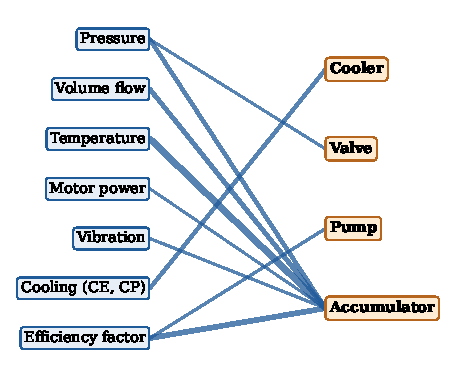
\includegraphics[width=\columnwidth]{rev_evidence_graph.pdf}
    \caption{Sensor-family evidence graph. An edge joins family $F$ and component $c$ when the mean family-level occlusion drop $w_{F,c}$ of \eqref{eq:edgeweight} is at least 0.01, and its width is proportional to $w_{F,c}$. The graph aggregates pooled out-of-fold predictions of the blocked split (seed 2026) and shows model sensitivity, not causal or physical support.}
    \label{fig:evidencegraph}
\end{figure}

\begin{figure*}[!t]
    \centering
    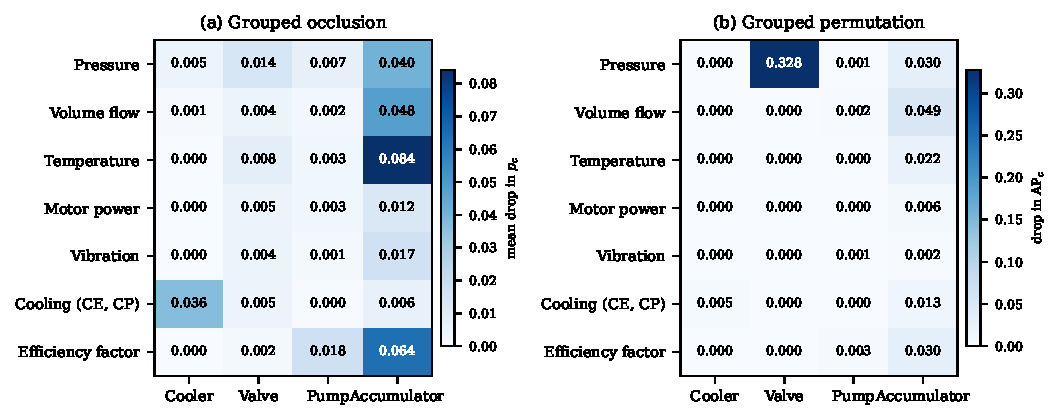
\includegraphics[width=0.85\textwidth]{rev_family_importance.pdf}
    \caption{Family-level attributions on the blocked split (seed 2026, weighted
    mean over folds). (a) Mean drop in $p_c$ when the family is mean-imputed.
    (b) Drop in average precision when the family is permuted.}
    \label{fig:importance}
\end{figure*}

These values describe how the fitted model responds to artificial inputs, and their stability is limited (Table~\ref{tab:stability}). Across ten fits (five blocked
folds and two seeds), channel-level occlusion rankings agree with median Spearman
correlation 0.30 to 0.60, with negative minima for three components. Family-level
occlusion is more stable for the pump and accumulator (median 0.75 and 0.79) than for
the cooler (0.26), whose vector is zero for most families. The modal top family is
the same in 60\% to 80\% of fits. SHAP rankings are stable across folds for three
components (median 0.81 to 0.87) but not for the accumulator (0.35), and occlusion
agrees with SHAP within a fold with median correlation 0.21 to 0.73. We therefore
read the graph as ordinal model-sensitivity evidence for the strongest edges and do
not attach a physical interpretation to individual edge weights.

\begin{table}[t]
\centering
\caption{Stability of the grouped attributions on the blocked split, given as the median (minimum) Spearman correlation between importance vectors. ``Fit vs.\ fit'' compares all pairs among ten fits, which are five folds with seeds 17 and 2026. SHAP rows use seed 2026 and 120 held-out cycles per fold. Pairs with a constant vector are excluded, which removes up to 38\% of permutation pairs for the cooler and accumulator because most of their groups have zero drop.}
\label{tab:stability}
\footnotesize
\setlength{\tabcolsep}{2pt}
\resizebox{\linewidth}{!}{%
\begin{tabular}{lrrrr}
\toprule
Comparison & Cooler & Valve & Pump & Accum. \\
\midrule
Occlusion, 17 channels, fit vs.\ fit & 0.35 (-0.35) & 0.30 (-0.27) & 0.60 (0.13) & 0.53 (-0.16) \\
Permutation, 17 channels, fit vs.\ fit & 0.36 (-0.29) & 0.32 (-0.03) & 0.54 (0.22) & -0.01 (-0.55) \\
SHAP, 17 channels, fold vs.\ fold & 0.87 (0.78) & 0.81 (0.66) & 0.87 (0.81) & 0.35 (-0.12) \\
Occlusion, 7 families, fit vs.\ fit & 0.26 (-0.68) & 0.54 (-0.43) & 0.75 (0.32) & 0.79 (0.36) \\
Permutation, 7 families, fit vs.\ fit & 0.68 (-0.25) & 0.59 (-0.04) & 0.68 (0.14) & 0.32 (-0.39) \\
Occlusion vs.\ SHAP, same fold & 0.21 (-0.17) & 0.50 (-0.26) & 0.73 (0.61) & 0.59 (-0.00) \\
Occlusion vs.\ permutation, same fold & 0.01 (-0.26) & 0.38 (0.08) & 0.39 (0.16) & 0.31 (-0.24) \\
\bottomrule
\end{tabular}}
\end{table}


\subsection{A Retrospective Example}
\label{sec:example}

The worked example of the original submission was chosen with the test labels and
had all four components faulted, so it could not show an ordering decision. We now select the case by a rule that uses no labels. It is the first held-out cycle, in recording
order, of the pooled blocked predictions for which exactly two components have
$p_c\ge0.5$ (597 cycles qualify). That is cycle index 6, in fold 0
(Fig.~\ref{fig:priority}), and only its cooler is faulted. The classifier gives $p_c$ of 0.524, 0.157, 0.012 and 0.924 for cooler, valve, pump and accumulator. Probability-only ranking and the priority score therefore both rank the healthy accumulator first ($M_c$ 2.161 against 1.169 for the cooler), and both are wrong on this cycle.
The example is a retrospective illustration of what an operator would be handed,
including a ranking error. It is not evidence that the ranking identifies the
component to inspect first.

\begin{figure}[!tbp]
    \centering
    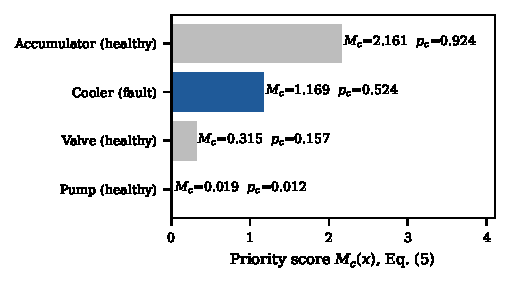
\includegraphics[width=\columnwidth]{rev_priority_example.pdf}
    \caption{Retrospective example selected without labels, as the first held-out cycle of the blocked split with exactly two components at $p_c\ge0.5$. Bars give the priority score of Eq.~\eqref{eq:priority}, and blue marks the truly faulted component. Both probability-only and priority ranking place the healthy accumulator first.}
    \label{fig:priority}
\end{figure}

\subsection{Agreement with a Third Attribution Method}
\label{sec:shapagree}

Table~\ref{tab:explainagree} reports Spearman correlations between occlusion,
permutation importance and grouped SHAP values (\texttt{TreeExplainer}
\cite{Lundberg2017SHAP}) across the 17 channel groups for one random-split fit.
Occlusion and SHAP agree for the valve, pump and accumulator ($\rho=0.640$ to
0.843) but not for the cooler ($\rho=-0.078$), and permutation importance tracks
neither well. This single-fit check is superseded as evidence of stability by the
fold-and-seed analysis of Table~\ref{tab:stability}, which shows weaker agreement
on the blocked split.

\begin{table}[t]
\centering
\caption{Spearman rank agreement, across the 17 sensor groups, between grouped occlusion, permutation importance, and grouped SHAP (\texttt{TreeExplainer}) attribution, per component. Random-split test set, one fit (seed 17). Stability across blocked folds and seeds is in Table~\ref{tab:stability}.}
\label{tab:explainagree}
\footnotesize
\setlength{\tabcolsep}{4pt}
\begin{tabular}{lrrr}
\hline
Component & Occl.--Perm. & Occl.--SHAP & Perm.--SHAP \\
\hline
Cooler & 0.000 & -0.078 & 0.476 \\
Valve & -0.212 & 0.787 & 0.000 \\
Pump & 0.190 & 0.843 & 0.298 \\
Accumulator & -0.184 & 0.640 & 0.290 \\
\hline
\end{tabular}
\end{table}


\subsection{Robustness Under Simulated Degradation}
\label{sec:degradationwalk}

To characterize how ranking degrades with data quality, we sweep four axes, each at
five levels, over 10 seeds (17, 2026, 101, 202, 303, 404, 505, 606, 707, 808). The evaluation fold is fixed at fold~0 of the ten-block split (blocks 0 and 9, 445 cycles).
The first axis is the training fraction retained, $\{1.0, 0.3, 0.1, 0.03, 0.01\}$.
The second removes $\{0,1,2,3,4\}$ of the seven families of Table~\ref{tab:channelmap},
chosen at random per seed. The third is the training-label flip rate,
$\{0,0.05,0.10,0.20,0.30\}$, applied per component after the split so test labels
stay clean. The fourth is the fraction of each cycle retained before feature
extraction, $\{1.00,0.50,0.25,0.10,0.05\}$. Each of the 200 fits reuses the headline
forest and policies (Fig.~\ref{fig:degradationwalk}, Table~\ref{tab:degradationwalk}).

Table~\ref{tab:reconcile} reconciles this sweep with Table~\ref{tab:ceilingbound}.
The undegraded row of the sweep reports top-1 accuracy 0.978 for the priority score,
whereas Table~\ref{tab:ceilingbound} reports error 0.051 (accuracy 0.949). The two tables report different values because they evaluate different test sets. On fold~0 alone, probability-only and the
priority score both reach 0.978 for every seed; the priority score's excess error
comes from the other four folds, and on the pooled five folds it is present for every
seed. The macro-F1 of 0.961 in the sweep is likewise the fold-0 mean over ten seeds,
not the five-fold mean of 0.965.

Top-1 accuracy degrades less than macro-F1 on every axis. Retaining 5\% of each cycle lowers
macro-F1 from 0.961 to 0.791 while top-1 accuracy moves from 0.978 to 0.975.
Training-label noise degrades ranking most (top-1 0.942 at a 30\% flip rate), and
removing four of seven families has the smallest effect (0.976). Top-1 accuracy at
3\% of the training rows (about 53 cycles) already reaches 0.977; at 1\% (about 17
rows) the fit becomes unstable across seeds (mean 0.932, standard deviation 0.083).
Probability-only ranking never exceeds its bound in the sweep, as
Proposition~\ref{prop:bound}(i) requires. Local occlusion also stayed below $B_p$
in all twenty cells, but it violates the classifier's order on 1.1\% to 3.6\% of
fold-0 cycles across seeds, so that is an empirical observation and not a
consequence of the bound. The priority score exceeds $B_p$ in one cell (training
fraction 0.01; 0.068 against 0.065).

\begin{figure*}[!t]
    \centering
    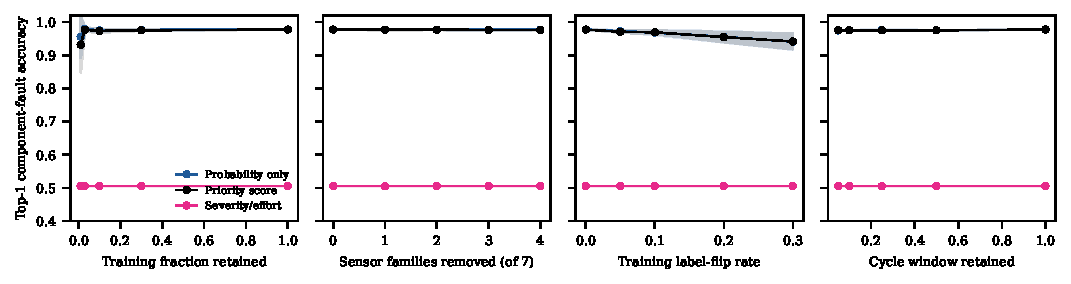
\includegraphics[width=0.85\textwidth]{degradation_walk.pdf}
    \caption{Top-1 component-fault accuracy under four degradation axes on fold~0 of the ten-block split, as the mean over 10 seeds with a shaded band of $\pm1$ standard deviation. Data are in \texttt{results/degradation\_walk\_summary.csv}.}
    \label{fig:degradationwalk}
\end{figure*}

\begin{table}[!t]
\centering
\caption{Degradation walk for the priority-score policy, with 10 seeds per level and the evaluation fixed at fold~0 of the ten-block split (blocks 0 and 9, 445 cycles). For each axis and level the table gives mean top-1 component-fault ranking accuracy, the union-bound top-1 error, mean cross-component AUC and macro-F1. Code is in \texttt{code/degradation\_walk.py} and data in \texttt{results/degradation\_walk\_summary.csv}.}
\label{tab:degradationwalk}
\footnotesize
\setlength{\tabcolsep}{3pt}
\resizebox{\linewidth}{!}{%
\begin{tabular}{llrrrr}
\hline
Axis & Level & Top-1 & Bound err.\ & Cross-AUC & Macro-F1 \\
\hline
Training fraction retained & 0.01 & 0.932 & 0.065 & 0.972 & 0.770 \\
Training fraction retained & 0.03 & 0.977 & 0.026 & 0.988 & 0.918 \\
Training fraction retained & 0.10 & 0.973 & 0.031 & 0.985 & 0.966 \\
Training fraction retained & 0.30 & 0.975 & 0.031 & 0.985 & 0.950 \\
Training fraction retained & 1.00 & 0.978 & 0.027 & 0.987 & 0.961 \\
\hline
Sensor families removed (of 7) & 0 & 0.978 & 0.027 & 0.987 & 0.961 \\
Sensor families removed (of 7) & 1 & 0.977 & 0.032 & 0.985 & 0.954 \\
Sensor families removed (of 7) & 2 & 0.977 & 0.033 & 0.985 & 0.943 \\
Sensor families removed (of 7) & 3 & 0.976 & 0.033 & 0.985 & 0.938 \\
Sensor families removed (of 7) & 4 & 0.976 & 0.038 & 0.983 & 0.910 \\
\hline
Training label-flip rate & 0.00 & 0.978 & 0.027 & 0.987 & 0.961 \\
Training label-flip rate & 0.05 & 0.971 & 0.043 & 0.980 & 0.945 \\
Training label-flip rate & 0.10 & 0.969 & 0.045 & 0.979 & 0.925 \\
Training label-flip rate & 0.20 & 0.955 & 0.056 & 0.974 & 0.894 \\
Training label-flip rate & 0.30 & 0.942 & 0.080 & 0.964 & 0.864 \\
\hline
Cycle window retained & 0.05 & 0.975 & 0.041 & 0.981 & 0.791 \\
Cycle window retained & 0.10 & 0.975 & 0.041 & 0.981 & 0.802 \\
Cycle window retained & 0.25 & 0.975 & 0.034 & 0.984 & 0.937 \\
Cycle window retained & 0.50 & 0.975 & 0.029 & 0.986 & 0.981 \\
Cycle window retained & 1.00 & 0.978 & 0.027 & 0.987 & 0.961 \\
\hline
\end{tabular}}
\end{table}

\begin{table}[t]
\centering
\caption{Reconciliation of the blocked-split top-1 figures. Table~\ref{tab:ceilingbound} pools the out-of-fold predictions of all five folds (2205 cycles, seed 2026), whereas the degradation sweep of Table~\ref{tab:degradationwalk} evaluates only fold~0 (blocks 0 and 9, 445 cycles) and averages ten seeds. The fold-0 columns give top-1 accuracy and the pooled columns give top-1 error.}
\label{tab:reconcile}
\footnotesize
\setlength{\tabcolsep}{3pt}
\begin{tabular}{rrrrr}
\toprule
Seed & Fold 0 acc. & Fold 0 acc. & Pooled err. & Pooled err. \\
 & prob.\ only & priority & prob.\ only & priority \\
\midrule
17 & 0.978 & 0.978 & 0.022 & 0.054 \\
2026 & 0.978 & 0.978 & 0.022 & 0.051 \\
101 & 0.978 & 0.978 & 0.025 & 0.056 \\
202 & 0.978 & 0.978 & 0.025 & 0.052 \\
303 & 0.978 & 0.978 & 0.021 & 0.053 \\
404 & 0.978 & 0.978 & 0.022 & 0.051 \\
505 & 0.978 & 0.978 & 0.026 & 0.050 \\
606 & 0.978 & 0.978 & 0.024 & 0.058 \\
707 & 0.978 & 0.978 & 0.024 & 0.056 \\
808 & 0.978 & 0.978 & 0.025 & 0.059 \\
\midrule
Mean & 0.978 & 0.978 & 0.024 & 0.054 \\
\bottomrule
\end{tabular}
\end{table}


\subsection{Classifier Comparators}
\label{sec:comparators}

We add two comparators to test whether the conclusions depend on the forest. The first is HistGradientBoosting (HGB) on the identical 187 features, with one binary model per component, and the second is a small 1-D convolutional neural network (CNN) on the 17 raw streams block-averaged to 60 samples per cycle. Table~\ref{tab:comparators} reports
them on the random split, on fold~0 of the blocked split, and on the chronological
split. On fold~0, HGB reaches macro-F1 0.967 against 0.962 for the forest, and the
1-D CNN is markedly worse on both harder splits (0.695 and 0.222).

\begin{table}[t]
\centering
\caption{Classifier comparators, given as mean $\pm$ standard deviation over the seeds 17, 2026 and 4242. The blocked row uses only fold~0 (blocks 0 and 9, 445 cycles), which is the fold of the degradation sweep, and pooled five-fold results for HistGradientBoosting are in Sec.~\ref{sec:comparators}. HistGradientBoosting without subsampling is deterministic, so its standard deviation is 0. It uses the same 187-feature cycle table as the random forest, while the 1-D CNN uses the 17 raw sensor streams block-averaged to a common 60 samples per cycle (Sec.~\ref{sec:comparators}). Mean cross-AUC and the union-bound top-1 error are computed as in Table~\ref{tab:ceilingbound}.}
\label{tab:comparators}
\footnotesize
\setlength{\tabcolsep}{3pt}
\resizebox{\linewidth}{!}{%
\begin{tabular}{llrrr}
\hline
Split & Classifier & Macro-F1 & Top-1 acc.\ & Mean cross-AUC \\
\hline
Random & Random Forest (headline) & 0.999 $\pm$ 0.000 & 1.000 $\pm$ 0.000 & 1.000 \\
Random & HistGradientBoosting & 0.999 $\pm$ 0.000 & 1.000 $\pm$ 0.000 & 1.000 \\
Random & 1D-CNN (raw, resampled 1 Hz) & 0.939 $\pm$ 0.010 & 0.993 $\pm$ 0.001 & 0.995 \\
\hline
Blocked 5-fold & Random Forest (headline) & 0.962 $\pm$ 0.003 & 0.978 $\pm$ 0.000 & 0.987 \\
Blocked 5-fold & HistGradientBoosting & 0.967 $\pm$ 0.000 & 0.982 $\pm$ 0.000 & 0.991 \\
Blocked 5-fold & 1D-CNN (raw, resampled 1 Hz) & 0.695 $\pm$ 0.074 & 0.901 $\pm$ 0.054 & 0.954 \\
\hline
Chronological & Random Forest (headline) & 0.645 $\pm$ 0.020 & 0.825 $\pm$ 0.000 & 0.750 \\
Chronological & HistGradientBoosting & 0.670 $\pm$ 0.000 & 0.958 $\pm$ 0.000 & 0.928 \\
Chronological & 1D-CNN (raw, resampled 1 Hz) & 0.222 $\pm$ 0.000 & 0.825 $\pm$ 0.000 & 0.695 \\
\hline
\end{tabular}}
\end{table}


Because similar classification scores need not imply similar rankings or
explanations, we repeated the ranking and attribution analyses with HGB on all five
blocked folds (\texttt{results/revision/hgb\_ranking\_blocked.csv}). Pooled over the
folds, HGB has a slightly lower fold-mean macro-F1 than the forest (0.959 against
0.965) but a lower probability-only top-1 error (0.010 against 0.022), and it again
attains its bound ($B_p=0.010$). Its priority score is much worse (0.105; paired
difference 0.095 [0.054, 0.154]), and local occlusion rises to 0.070. The direction
of the negative result is the same under both classifiers, and its size depends on
the classifier. HGB's family-level occlusion rankings correlate with the forest's at
$\rho=0.83$, 0.18, 0.43 and 0.68 for cooler, valve, pump and accumulator, and the
top family agrees for three components but not for the accumulator (efficiency
factor for HGB, temperature for the forest). Explanations are therefore
classifier-dependent, and we claim classifier independence only for the
classification scores and the direction of the ranking comparison.

\section{Discussion}
\label{sec:discussion}

The results support a narrower statement than the original submission made. Ranking by the classifier's probabilities beats static severity and effort
policies on every cross-validated protocol, and loses to them only at the early
chronological cuts, where the cooler model degenerates. Reweighting the probabilities by severity, effort and occlusion does not help. It hurts on the two
temporally blocked protocols, is neutral under profile holdout, and cannot be
rescued by choosing the weights on training blocks. Proposition~\ref{prop:bound} explains part of this result, since any order-preserving policy inherits the classifier's error budget, which is small here. A reweighting can beat probability-only ranking only by reordering components. The priority score does so on about half of the
cycles, and on these protocols the net effect of the reorderings is negative. Judging a score built to encode urgency by top-1 accuracy
measures its constants as much as its usefulness. A fair test of the priority score
needs a maintenance-utility criterion and cost data, which this benchmark does not
contain.

\subsection{Comparison with Published Results}
\label{sec:publishedcomparators}

The data set's documentation reports two prior studies on these four labels.
Helwig et al.\ \cite{Helwig2015Hydraulic} found the cooler and valve states easy to
classify and the pump and especially the accumulator harder. Schneider et al.\
\cite{Schneider2017FeatureExtraction} targeted the accumulator with automatic feature
extraction and selection and reported a large reduction in its error rate. Both
studies report accuracy or error under protocols that differ from ours, so their
figures are not comparable with our F1 scores, and Table~\ref{tab:publishedcomparators}
compares only the qualitative pattern. In our leakage-controlled per-component F1
(Table~\ref{tab:splitcompare}) the accumulator is the hardest component, as in both studies, at about 0.89. The cooler, valve and pump all exceed 0.96, so the pump, which Helwig et al.\ found harder, is easy under our features. A controlled comparison would require
reproducing those methods under our label mapping and protocols, which we have not
done.

\begin{table}[!t]
\centering
\caption{Qualitative comparison with two prior studies on the same benchmark.
Prior studies used different metrics and protocols, so no numeric comparison is
made.}
\label{tab:publishedcomparators}
\footnotesize
\setlength{\tabcolsep}{3pt}
\begin{tabularx}{\columnwidth}{@{}l
  >{\raggedright\arraybackslash}X
  >{\raggedright\arraybackslash}p{0.38\columnwidth}@{}}
\toprule
Component & Prior studies \cite{Helwig2015Hydraulic,Schneider2017FeatureExtraction} & This paper, leakage-controlled (Table~\ref{tab:splitcompare}) \\
\midrule
Cooler & easy target & among the easiest \\
Valve & easy target & easy; sensitive to purging \\
Pump & harder target & easy \\
Accumulator & hardest target; focus of feature selection & hardest under every protocol \\
\bottomrule
\end{tabularx}
\end{table}

\section{Limitations and Threats to Validity}
\label{sec:limitations}

\subsection{Benchmark Separability}
\label{sec:benchmarkseparability}

After cycle-level feature extraction the component states separate readily, and
under profile holdout the probability-only error is 0.006. A benchmark this
separable leaves little room for any ranking policy to improve on the classifier,
and Proposition~\ref{prop:bound} makes the room computable from cross-component AUC.
Separating the priority formula from probability-only ranking requires field data
with drifting sensors, incomplete labels, ambiguous interactions and cost records.

\subsection{Target Definition and Causal Scope}

The labels say which components are degraded, not which degradation caused the
others, so the ranking task is component-fault ranking and nothing here identifies a
root cause. The evidence graph summarizes model sensitivity under mean imputation.
It does not identify causal mechanisms or physical support \cite{Pearl2009Causality},
its attributions inherit the known biases of removal-based methods
\cite{Strobl2007Bias,Hooker2021Unrestricted}, and their stability across folds is
moderate at best.

\subsection{Maintenance Decision Modeling}

The severity and effort constants are illustrative and fixed. Before operational
use they should be elicited from domain experts or estimated from downtime, safety,
cost and repair-time records using established multi-criteria methods
\cite{Saaty1980AHP,Braglia2000MAFMA,Liu2013FMEAReview}, and the score should be
evaluated against expected maintenance cost rather than top-1 accuracy.

\subsection{Generalization and Reporting}

The leakage-controlled protocols establish performance on held-out runs and unseen
fault combinations of one laboratory rig. They do not establish performance under
future operation, at unseen severity levels, or on another asset. The chronological
split is a stress test with degenerate per-component scores. The raw probabilities are
poorly calibrated for the accumulator and valve on held-out data, and the reported
calibration of the random split is a best case.

\section{Conclusion}
\label{sec:conclusion}

This paper evaluates explainable component-fault ranking on a public hydraulic
benchmark under protocols that control leakage. The classifier generalizes to held-out
runs and unseen fault combinations of the rig (macro-F1 0.962 to 0.965). The proposed
priority weighting does not improve on probability-only ranking. It is worse on both
temporally blocked protocols (paired differences 0.029 and 0.021), indistinguishable
under profile holdout, and not rescued by nested weight selection. A union bound on
top-1 error, valid for every ranking that preserves the classifier's per-cycle order,
shows how much room the classifier leaves for ranking policies to differ, and the
reweighted scores fall outside it because they reorder components. The attributions
are reported as model-sensitivity evidence with moderate stability. Future work should
test the priority score against a maintenance-cost criterion on field data with
recorded repair costs and genuine shift across assets.

\section*{Declarations}

\textbf{Data availability.} The UCI Condition Monitoring of Hydraulic Systems data
set analyzed here is publicly available \cite{Helwig2015Hydraulic,Dua2019UCI}; no new
data were collected. SHA-256 digests of the 17 sensor files and \texttt{profile.txt}
used in this study are recorded in the deposit manifest.

\textbf{Code availability.} The analysis code, generated tables, result files and cached
out-of-fold predictions behind every reported number are archived at
\url{https://doi.org/\depositdoi} and mirrored at \url{\repourl}. Installation
instructions, library versions and the order in which the scripts run are documented
in the deposit's \nolinkurl{HOW_TO_INSTALL_AND_REPRODUCE.md}.

\textbf{Funding.} This research received no external funding.

\textbf{Competing interests.} The author declares no competing interests.

\textbf{Author contributions.} Imran: Conceptualization, Methodology, Software,
Validation, Formal analysis, Investigation, Data curation, Writing (original draft,
review and editing), Visualization, Project administration.

\section*{Acknowledgment}

Generative AI tools (Claude, Anthropic) were used to assist with language editing
of the manuscript and with drafting, refactoring and running parts of the research
code, including the analyses added in revision. All AI-assisted text and code were
reviewed and checked by the author, who takes full responsibility for the content of
this article, the correctness of the reported experiments, and the integrity of the
released software.

\bibliographystyle{IEEEtran}
\bibliography{references}

\end{document}
